\documentclass{article}
%\documentclass[twocolumn]{article}
%\documentclass[onecolumn]{article}
% \usepackage{scrtime} % for \thistime (this package MUST be listed first!)
\DeclareUnicodeCharacter{0301}{\'{e}}
\usepackage{float}
\usepackage{times}
\usepackage{graphicx}
\usepackage{float}
\usepackage[margin=0.75in]{geometry}
\usepackage{fancyhdr}
\usepackage{caption}
\usepackage{notoccite}
\usepackage{pgfplotstable}
%\usepackage[round]{natbib}
%\setcitestyle{aysep={}} %removes the comma between the author and year in citations
%\usepackage{underscore}
\usepackage{pdfpages}
\usepackage{xcolor,colortbl}%for changing cell colour
\usepackage[normalem]{ulem}
\useunder{\uline}{\ul}{}
\usepackage{xspace}
\usepackage{booktabs}
\usepackage{capt-of}
\pagestyle{fancy}
\setlength{\headheight}{15.2pt}
\setlength{\headsep}{13 pt}
\setlength{\parindent}{28 pt}
\setlength{\parskip}{12 pt}
\pagestyle{fancyplain}
\usepackage[T1]{fontenc}
\usepackage{amsmath}
% \usepackage{color,amsmath,amssymb,amsthm,mathrsfs,amsfonts,dsfont}
\usepackage{xspace}
\usepackage{tikz-cd}
\usepackage{tikz}
\usetikzlibrary{decorations.markings}
\usetikzlibrary{calc, arrows}
\usetikzlibrary{external}
\usepackage{pgfplots}
\pgfplotsset{layers/my layer set/.define layer set={background,main,foreground}{},
        set layers=my layer set,}

\usepackage{listings}
\usepackage{xcolor}

\definecolor{codegreen}{rgb}{0,0.6,0}
\definecolor{codegray}{rgb}{0.5,0.5,0.5}
\definecolor{codepurple}{rgb}{0.58,0,0.82}
\definecolor{backcolour}{rgb}{0.95,0.95,0.92}

%for code
\lstdefinestyle{mystyle}{
	backgroundcolor=\color{backcolour},   
	commentstyle=\color{codegreen},
	keywordstyle=\color{magenta},
	numberstyle=\tiny\color{codegray},
	stringstyle=\color{codepurple},
	basicstyle=\ttfamily\footnotesize,
	breakatwhitespace=false,         
	breaklines=true,                 
	captionpos=b,                    
	keepspaces=true,                 
	numbers=left,                    
	numbersep=5pt,                  
	showspaces=false,                
	showstringspaces=false,
	showtabs=false,                  
	tabsize=2
}

\lstset{style=mystyle}
% \usetikzlibrary{pgfplots.clickable}
% \usepgfplotslibrary{clickable}
% tables
\usepackage{longtable}
\usepackage{booktabs}
\usepackage{multicol}
\usepackage{multirow}
% figs
%\usepackage{subfig}% http://ctan.org/pkg/subfig
\usepackage{subcaption}
%\newsubfloat{figure}% Allow sub-figures
\usepackage{caption}%lable fig caption as fig
%\captionsetup[subfigure]{labelfont=bf, justification=raggedright, labelformat=empty} %no caption label
\usepackage{stackengine} %places caption inside figure?
\captionsetup{subrefformat=parens} %when you reference the subcaption it will be (a) for example %{labelfont={color=blue}}
%\captionsetup[subfigure]{labelsep=colon}


% \usepackage{acronym}
% \usepackage{lineno}%for line numbers
%%%%%%%%%%%%%%%%%%%%%%%%%%%%%%%%%%%%%%%%%%%%%%%%%%%%%%%%%%%%%%%%%%%%%%%%%%%%%%%%
% BIBLIOGRAPHY
%%%%%%%%%%%%%%%%%%%%%%%%%%%%%%%%%%%%%%%%%%%%%%%%%%%%%%%%%%%%%%%%%%%%%%%%%%%%%%%%
\usepackage[backend=biber, giveninits=true, doi=false, isbn=false, natbib=true, url=true, eprint=false, style=authoryear-comp, sorting=nyt, sortcites=ynt, maxcitenames=2, maxbibnames=10, minbibnames = 10, uniquename=false, uniquelist=false, dashed=false]{biblatex} % can change the maxbibnames to cut long author lists to specified length followed by et al., currently set to 99.

%% bibliography for each chapter...
\DeclareFieldFormat[article,inbook,incollection,inproceedings,patent,thesis,unpublished]{title}{#1\isdot} % removes quotes around title
\renewbibmacro*{volume+number+eid}{%
	\printfield{volume}%
	%  \setunit*{\adddot}% DELETED
	\printfield{number}%
	\setunit{\space}%
	\printfield{eid}}
\DeclareFieldFormat[article]{number}{\mkbibparens{#1}}
%\renewcommand*{\newunitpunct}{\space} % remove period after date, but I like it. 
\renewbibmacro{in:}{\ifentrytype{article}{}{\printtext{\bibstring{in}\intitlepunct}}} % this remove the "In: Journal Name" from articles in the bibliography, which happens with the ynt 
\renewbibmacro*{note+pages}{%
	\printfield{note}%
	\setunit{,\space}% could add punctuation here for after volume
	\printfield{pages}%
	\newunit}    
\DefineBibliographyStrings{english}{% clears the pp from pages
	page = {\ifbibliography{}{\adddot}},
	pages = {\ifbibliography{}{\adddot}},
} 
\DeclareFieldFormat{journaltitle}{#1\isdot}
\renewcommand*{\revsdnamepunct}{}%remove comma between last name and first name
\DeclareNameAlias{sortname}{family-given}
% \DeclareNameAlias{sortname}{last-first}
\renewcommand*{\nameyeardelim}{\addspace} % remove comma in text between name and date
\addbibresource{ABC1.bib} % The filename of the bibliography
\usepackage[autostyle=true]{csquotes} % Required to generate language-dependent quotes in the bibliography
\renewrobustcmd*{\bibinitperiod}{}
% you'll have to play with the citation styles to resemble the standard in your field, or just leave them as is here. 
% or, if there is a bst file you like, just get rid of all this biblatex stuff and go back to bibtex. 
%%%%%%%%%%%%%%%%%%%%%%%%%%%%%%%%%%%%%%%%%%%%%%%%%%%%%%%%%%%%%%%%%%%%%%%%%%%%%%%%
%
% generally hyperref needs to be loaded last
\usepackage[hidelinks,colorlinks=true,linkcolor=blue,citecolor=blue,urlcolor=darkbrown]{hyperref}
%\usepackage[hidelinks,colorlinks=false,citecolor=blue,urlcolor=darkbrown]{hyperref}
\tikzexternalize

\lhead{Cells at War: Game-Based Learning} %This needs to change
\rhead{Alexander Turco and Rosa da Silva}
\title{\sc Cells at War: The Playfulness of Game-Based Learning}
\author{\sc Alexander Turco and Rosa da Silva}

\providecommand{\figref}[1]{(Figure \ref{#1})}  %what?
\providecommand{\tabref}[1]{(Table \ref{#1})}  %what?
\providecommand{\e}[1]{\ensuremath{\times 10^{#1}}}
\newcommand{\seg}{\texttt{Seg}\xspace}
\newcommand{\ecoli}{\mbox{\textit{E.\,coli}}\xspace}
\newcommand{\sclong}{\textit{Saccharomyces cerevisiae}\xspace}
\newcommand{\scshrt}{\mbox{\textit{S.\,cerevisiae}}\xspace}
\newcommand{\sce}{\mbox{\textit{S.\,cerevisiae}}\xspace}
\newcommand{\hslong}{\textit{Homo sapiens}\xspace}
\newcommand{\hsshrt}{\mbox{\textit{H.\,sapiens}}\xspace}
\newcommand{\hse}{\mbox{\textit{H.\,sapiens}}\xspace}
\newcommand{\celong}{\textit{Caenorhabditis elegans}\xspace}
\newcommand{\ceshrt}{\mbox{\textit{C.\,elegans}}\xspace}
\newcommand{\dmlong}{\textit{Drosophila melanogaster}\xspace}
\newcommand{\dmshrt}{\mbox{\textit{D.\,melanogaster}}\xspace}
\newcommand{\atlong}{\textit{Arabidopsis thaliana}\xspace}
\newcommand{\atshrt}{\mbox{\textit{A.\,thaliana}}\xspace}
\newcommand{\pflong}{\textit{Plasmodium falciparum}\xspace}
\newcommand{\pfshrt}{\mbox{\textit{P.\,falciparum}}\xspace}

%%%%BIBLIOGRAPHY

%Supplementary File Table Numbers:
\newcommand{\expdata}{S1\xspace}
\newcommand{\seqdata}{S2\xspace}
\newcommand{\protdata}{S3\xspace}
\newcommand{\blast}{S4\xspace}
\newcommand{\tabvar}{S5\xspace}
%Supplementary File Fig Numbers:

\newcommand{\expcor}{S1\xspace}
\newcommand{\expdistATCC}{S3\xspace}
\newcommand{\specialcell}[2][c]{%
	\begin{tabular}[#1]{@{}c@{}}#2\end{tabular}}
\newcommand{\beginsupplement}{%
	\setcounter{table}{0}
	\renewcommand{\thetable}{S\arabic{table}}%    %thetable references table counter 
	\setcounter{figure}{0}
	\renewcommand{\thefigure}{S\arabic{figure}}%
	\setcounter{equation}{0}
	\renewcommand{\theequation}{S\arabic{equation}}%

}
\renewcommand{\thesection}{}
\renewcommand{\thesubsection}{}
\renewcommand{\thesubsubsection}{}
\usepackage{setspace}
%adjust spacing
\doublespacing
\usepackage{titlesec}

\titlespacing\section{0pt}{12pt plus 2pt minus 2pt}{0pt plus 1pt minus 1pt}
\titlespacing\subsection{0pt}{12pt plus 2pt minus 2pt}{0pt plus 1pt minus 1pt}
\titlespacing\subsubsection{0pt}{12pt plus 2pt minus 2pt}{0pt plus 1pt minus 1pt}

% below 3 lines will put ALL table captions at the top...not sure if
% this is what we want but it is good enough for now

% \usepackage{float}
\floatstyle{plaintop}
\restylefloat{table}
%%%%%%%%%%%%%%%%%%%%%%%%%%%%%%%%%%%%%%%%%%%%%%%%%%%%%%%%%%%%%%%%%%%
        
        \definecolor{atomictangerine}{rgb}{1.0, 0.6, 0.4}
        \definecolor{darkbrown}{rgb}{1.0, 0.56, 0.24}
        \colorlet{darkcol}{black!30!white}
        \colorlet{lightcol}{black!10!white}
        \definecolor{txtcol}{HTML}{F40000}


%%%%%%%%%%%%%%%%%%%%%%%%%%%%%%%%%%%%%%%%%%%%%%%%%%%%%%%%%%%%%%%%%%%
\begin{document}

\widowpenalty10000
\clubpenalty10000

%\linenumbers %for line numbers
\onecolumn
%\twocolumn[  
%       \begin{@twocolumnfalse}
%               \begin{center}
                        \maketitle
%               \end{center}
%                       \bigskip

\thispagestyle{empty}
\noindent \textsuperscript{1} Department of Biology, McMaster University, Hamilton, ON, Canada

\newpage
\tableofcontents
\newpage

\section{Abstract}

After many years of trying to adapt to educational innovations of the 21st Century, educators will soon be looking into the not-too-distant future to consider what modern learning in post-secondary education will look like in the 22nd Century. Technological advances will continue to transform the landscape of the classroom. The use of digital games, although a source of controversy and debate, will prove to be highly effective instructional tools that will promote problem solving and critical thinking skills. Their use has already started to change the structure of the class in the elementary classroom as they serve to energize and engage students in their learning and improve conceptual understandings, creativity, and imagination. The traditional construct of the classroom has started to evolve, embracing a new way in which knowledge, skills, and attitudes can be acquired. The primary focus of this study was to create and implement a biological video game that focused on a single gene disease, which served as a vehicle to teach cellular and molecular biology concepts. ‘Cells at War’ is a collection of scientific video games developed through interdisciplinary efforts that reinforces the notion that video games are highly effective tools used to enhance instructional methods and engage students in the biology classroom.

\newpage
       
\section{Literature Review/Proposal}

\subsection{Gamification of Learning}

Although the use of technology has become prevalent in schools across Canada, using game-based learning as an instructional approach is still in its infant stages. Educators are reticent to embrace digital technology and gaming as the new norm in the classroom due to insufficient technical competence, as well as challenges they face in selecting appropriate games \citep{jaaska2022teachers,molin2017role}. In addition, educators are rarely involved in the development of these games, making it difficult to facilitate suitable learning in the classroom \citep{molin2017role}. 

Kindergarten classrooms in Ontario are bustling places of activity, reflective of active inquiry through play. Exploration and provocations drive their curiosity while simultaneously developing their oral language and critical thinking skills \citep{kindergartencurriculum}. We believe that play is paramount for children in their formative years and educational theorists like Vygotsky affirm this. He was firm in his belief that play is the leading line of development during preschool years \citep{vygotsky1967play}. Unfortunately, in many classrooms, educators continue to feel more comfortable engaging in antiquated and traditional methods of instruction that consist of a didactic approach to learning. Some educators may be fearful that incorporating game-based learning into the curriculum will undermine their authority in the classroom \citep{jaaska2022teachers,chee2014facilitating,jong2016teachers}. The need to challenge current educational practices is paramount as it appears some educators are currently teaching students from the perspective of their own past rather than the realities of the students’ future. 

\subsection{What Happens to Play Beyond the Formative Years?}

The need to engage and motivate learners does not cease to be a need in a student’s educational career. However, what does become a priority in higher academic years are measurable student outcomes \citep{ball2012politics,shore2010beyond,leather2021pedagogy}. Tests and quizzes take precedence over the formative process of learning. Assessment of learning (tests and quizzes) dominates an educator’s instructional practices which in turn diminishes the value of the experiential learning process (assessment as learning). Assessment methods seem to be based on antiquated teaching practices, which have been influenced by our Victorian educational heritage that is rooted in a persistent view of fear of play \citep{wood2013play}. This rigidity in instructional norms appears to have taken hold in our classrooms which diminishes the value and importance of games in the classroom. \citet{reich2020failure} argues that schools are complex and conservative institutions that have little incentive to adopt or test novel approaches. 

It can be argued that this fear of play is also due in large part to limited resources and training being provided to educators \citep{fishman2014empowering}. Teachers require technological and pedagogical supports to develop their understanding of game based learning in the classroom. The expectation therefore to incorporate new and innovative teaching methodologies in the classroom is unrealistic without providing teachers with the appropriate training needed to do so. Incorporating game based learning in teacher practice is impacted by a lack of professional development opportunities that can systematically guide them in using games for teaching, learning, and assessment \citep{fishman2014empowering,ruggiero2013video,foster2020principles}. In order to develop teacher proficiency in game-based learning, further professional development is required in the form of pedagogical training in order to understand how to develop and utilize game-based learning practices.


\subsection{Do Games Help or Hurt Learning: The Debate Over Game-Based Learning}

The debate of whether game based learning helps or hinders learning is ongoing. What comes into question in opposition to game based learning is that it serves to act as a source of entertainment and amusement rather than for educative purposes \citep{lister2015gamification, mayer2010adding}. Many individuals associate play with children, and therefore believe that play is trivial and unimportant \citep{prensky2001fun}. It appears one does not learn to play, but rather plays to learn. Play is where a spark is ignited and the source in which curiosity is peaked. It is not silly, trivial or irrelevant but has a biological and evolutionary function which has a strong connection to learning \citep{prensky2001fun}. It is, as Danny Hillis, founder of Thinking Machines and a former Disney Fellow has stated something every single culture does \citep{prensky2001fun}.

Arguing the merits behind the development and creation of digital games for use in post-secondary classrooms can appear effortless. However, what cannot be overlooked at times is that educators spend a great deal of time planning and executing engaging lessons which can become time consuming and onerous. \citet{mckeachie2013mckeachie} argue that the biggest barrier to the use of games therefore is logistic. Although games can be fun and engaging, we know that our classrooms today are comprised of diverse students with varying needs and a one size fits all approach does not work.

\subsection{The Benefits of Using Video Games at the Post-secondary Level}

 Rules, goals and objectives, outcomes, competition, interaction, and story are what Mark Prensky refers to as the six key structural elements of games \citep{prensky2001fun}. These powerful factors are what set games apart from other engaging activities. Traditional forms of educational media lack what video games provide, a high degree of interactivity \citep{coller2009effectiveness}. Video games challenge individuals to work within specific parameters and respond to situations that occur in the game \citep{coller2009effectiveness}. The way in which individuals respond to challenges presented in video games allows them to think critically, strategize, and work collaboratively in an interactive and engaging manner.

Video games are visually appealing, stimulating, and heighten our senses in many ways. We become addicted to the hormone boost our brains receive when we achieve results \citep{tomavska2022let}. They allow us to learn through doing and creating. Like play, upon beginning a video game, one is completely immersed into a whole new world without boundaries \citep{coller2009effectiveness}. Each player is engaged in a creative process where they are free to discover the limitless possibilities contained within the game. In a school setting, we are often taught there is one solution or right answer or way of doing something. Video games challenge this by giving players multiple entry points and pathways to consider.

The growing evidence of the effectiveness of video games in the classroom is emerging, and the value of game based learning is evident throughout various disciplines. In 2005, Northern Illinois University began teaching an undergraduate course in Numerical Methods using a video game called “NIU-Torcs” \citep{coller2009effectiveness}. Students were observed spending twice the average amount of time on coursework than other subject areas \citep{coller2009effectiveness}. Other games are being developed for nursing education which focus on developing medication calculation skills. This is an area of global concern perhaps due to test anxiety and low mathematical self-efficacy in nursing students \citep{foss2013medication}. Further, as a result of the COVID-19 pandemic, educators were compelled to find alternative ways to supplement hands-on learning experiences in an online setting. In a study completed at McMaster University, virtual reality (VR) headsets were used to engage in a 3D laboratory simulation which allowed for open-ended investigations in a range of STEM fields such as chemistry, biology, and physics \citep{tsirulnikov2023game}. \citet{tsirulnikov2023game} noted higher levels of engagement and motivation through these VR simulations. Game based learning not only provides students with infinite possibilities for discovery but sustains student interest, builds confidence, and helps to improve cognition and learning outcomes \citep{divjak2011impact}.

The long-term positive effects of Game-Based Learning will continue to be researched and studied. Although empirical evidence is slowly emerging but still limited, studies and research to date are proving that Game-Based Learning has the potential to transform post secondary classrooms. A learning environment in which students are able to take risks, explore, discover, fail and try again is achieved through a collaborative and interactive process between student and teacher.

\section{Materials and Methods}

\subsection{Study Setting and Context}

Results from this study were obtained utilizing a first-year cellular and molecular biology course (BIO1A03) at McMaster University (Ontario, Canada). BIO1A03 provides first year students with a strong cell and molecular biology foundation that is required for most upper level courses in the Faculty of Science at McMaster. Enrollment in BIO1A03 tends to be high, with approximately 700 students taking the course during both the fall (September-December) and winter (January-April) semesters. Due to the lengthy process of video game design, we were limited to collecting data solely from students enrolled in the winter semester for this study.

It is worthwhile to note the current course format of BIO1A03. Prior to 2014, BIO1A03 followed a traditional, didactic format, which consisted of three 50 minute in-person lectures per week, accompanied by a bi-weekly, three-hour laboratory session \citep{tahir2022blended}. In 2013, BIO1A03 was converted into a Blended Learning course format, which included independent, self-paced learning through prerecorded modules, and face-to-face learning in the classroom with a heavier focus on student collaboration and engagement \citep{tahir2022blended}. Course content previously delivered during lecture was condensed into two weekly modules which students were required to complete prior to attending in-person lectures. In-person lectures were restructured and minimized to two per week. One of these sessions consisted of a review lecture, where students could clarify concepts they found difficult to understand, while the other focused on applying theoretical concepts that students had learned to a real world concept. In a study highlighting the impacts of blended learning in BIO1A03 at McMaster, \citet{tahir2022blended} noted that the majority of students surveyed after taking the course felt that these novel blended learning approaches enabled them to improve general knowledge and understanding of core concepts in cellular and molecular biology.

\subsection{Video Game Design/Creation}

The conversion to a blended learning approach in BIO1A03 allowed for a seamless transition to online-learning in 2019 when the COVID-19 pandemic began. During this time, the BIO1A03 instructional team began exploring other novel pedagogical approaches which could help improve student learning. The idea of using digital games to improve education has been around for quite some time, however the controversy surrounding video games in this context is still apparent.

In 2021, the BIO1A03 instructional team partnered up with the George Brown College School of Design, and received support from CEWIL Canada (Co-operative Education and Work-Integrated Learning Canada), formerly known as CAFCE (Canadian Association for Co-operative Education), to design and implement an educational biological video game that could be used as an instructional and engaging teaching tool in BIO1A03. A small cohort of McMaster Univeristy Biology students and supervising professors, as well as game designers, programmers, animators, audio engineers, and artists from the George Brown College School of Design were selected to pilot this work-integrated learning project.

Concept development began in September of 2021. In this phase, students from both institutions worked collaboratively to brainstorm concepts for a biological video game that would be both engaging and educational. The theme for the game was centred around single-gene diseases. Biology students from McMaster University were responsible for selecting and researching a specific single-gene disease. This information was exchanged with students from George Brown College, who in-turn provided a wealth of knowledge on how to turn these static, difficult to understand concepts into engaging gameplay mechanics. Students pitched these proposals to supervising professors who then selected the ideas and game elements that best suited the goals of the project.

The game production phase then began in November of 2021. Students from George Brown College started bringing these ideas to life through artwork, animation, and programming. McMaster Biology students served as subject matter experts, ensuring scientific accuracy throughout the production process, as well as creating an encyclopedia of important biological concepts that were highlighted in-game. Throughout the production stage, weekly online meetings were held to keep all members updated with progress. Discord was also utilized throughout the entire process in order to ensure open dialogue between students and supervisors, as well as to share game assets and important information. A functioning build of the game was completed in late March of 2021, and was introduced in the final BIO1A03 class of the winter 2021 semester, in place of lecture material. After class, students were asked to complete a survey regarding their attitudes towards the game.

\subsection{Study Participants}

Students qualifying for participation in the survey included only those enrolled in the winter 2021 semester of BIO1A03. Students were informed about the survey prior to playing the game, through both in-class and online announcements posted on Desire to Learn. Students who did not complete the survey were informed that this would not effect course performance. Those who participated were incentivized by being entered into a draw to win prizes.

\subsection{Survey Design: Qualitative Analysis of Student Feedback NOT DONE YET}

The survey was developed and delivered through the LimeSurvey\textregistered \space platform. Students were asked a total of 14 questions regarding opinions and attitudes on their current undergraduate education, as well as feedback on game-based learning in the biology classroom. The National Survey of Student Engagement (NSSE) was used as a framework to generate the questions that were asked. NSSE questions assess the extent to which students engage in educational practices in the context of higher levels of learning (NSSE website citation). MORE HERE ABOUT NSSE...

\section{Results}

\subsection{Student perceptions of current undergraduate experiences}

150 students enrolled in the winter 2021 session of BIO1A03 attended a game-based style lecture and completed the follow-up survey. Students were presented with condensed lecture material prior to completing the relevant level in the game. The idea behind this was to provide a brief introduction of the content to students, and then allow them to further explore these concepts by playing the game. 

Participants were asked a series of questions regarding their current experiences as undergraduate science students, as well as questions regarding the benefits of implementing game-based learning approaches into their classrooms. To gain insight into how experience students had playing video games, they were asked to indicate a weekly average amount of time spent playing them \figref{fig:1}. 66 Participants (44\%) indicated that they did not play video games, while 53 participants (36\%) indicated that they spent between 1-10 hours per week. Only 7 students (5\%) were found spending approximately 10-20 hours per week playing video games. It is interesting to note that participants who reported not playing video games also emphasized that the game was `easy to navigate' and `very accessible'. This suggests that a lack of experience playing video games did not necessarily limit students' abilities to learn course content through playing the game.

%%%%%TIME SPENT PLAYING VIDEO GAMES
\begin{figure}[H]
	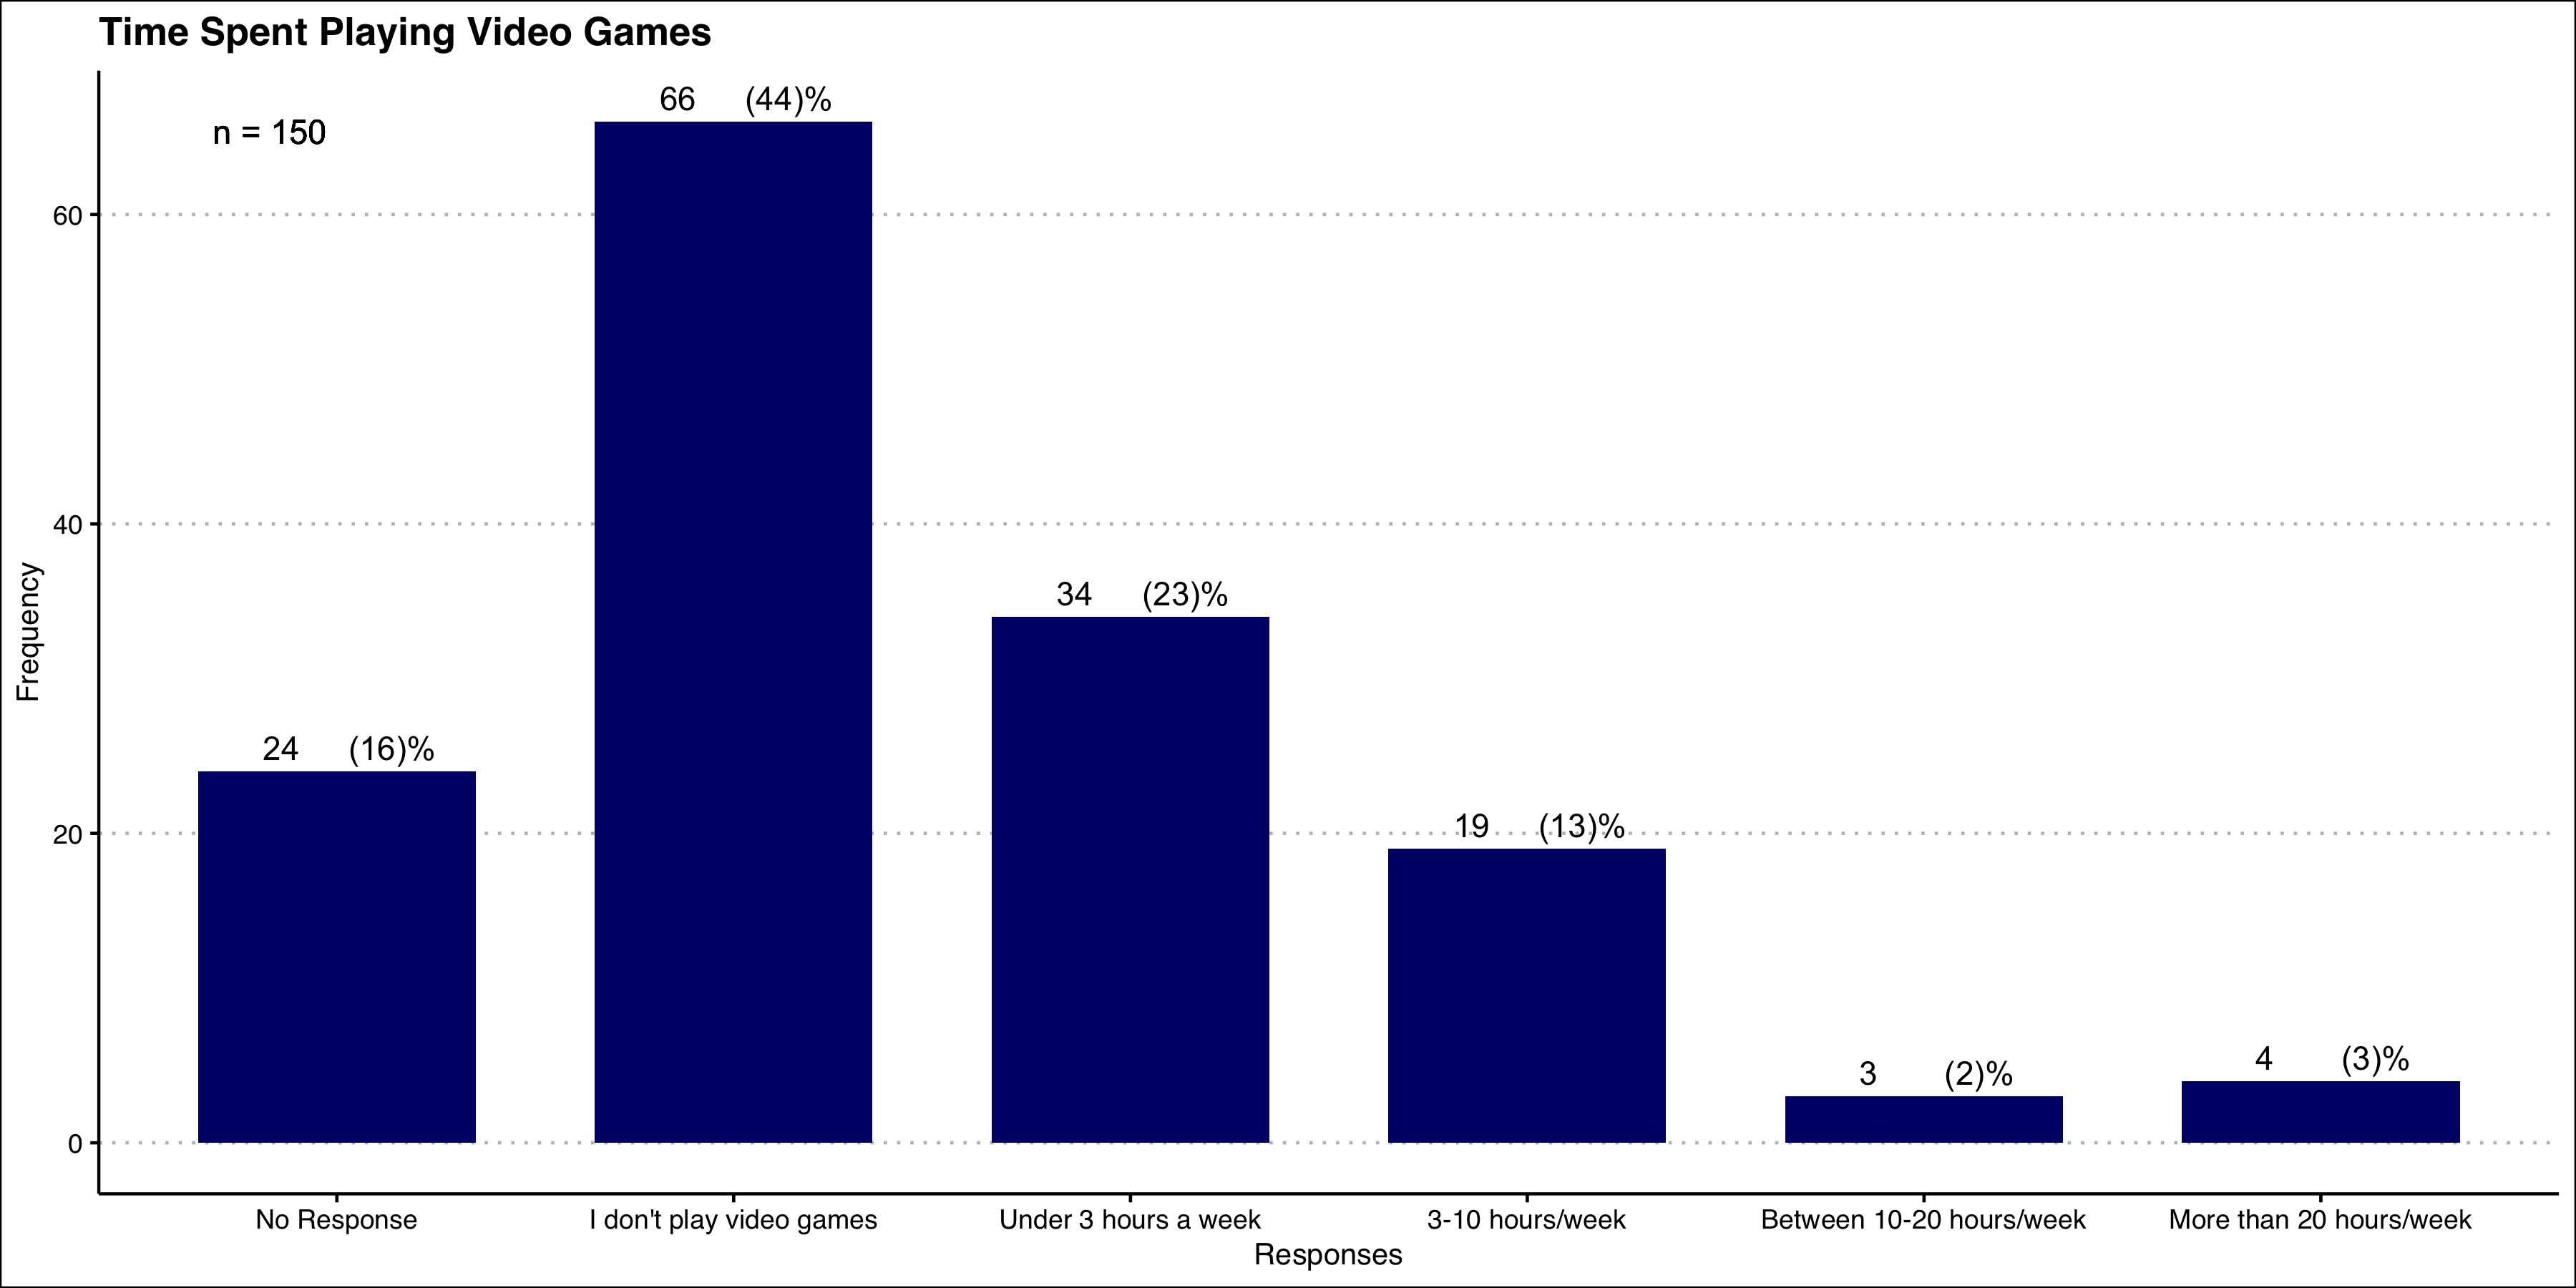
\includegraphics[width=\textwidth]{figures_4f06/time_spent_playing_videogames.jpg}
	\caption{Student responses regarding the average amount of weekly time spent playing video games}
	\label{fig:1}
\end{figure}

Further data obtained provided insight into the various types of courses students were taking at McMaster University during the fall/winter 2021 semesters \figref{fig:2}. At this time, McMaster University was slowly shifting back to in-person classes due to COVID-19 restrictions being lifted, however, a large majority of courses had been converted to hybrid, blended learning, and online courses. 60 participants (40\%) indicated that the majority of courses they were taking were mostly hybrid or blended learning style courses. 28 participants (19\%) indicated most of their courses were back in-person, while only 7 participants (5\%) were enrolled in mostly online courses. 30 participants indicated a balanced mix of all course types. These results highlight the shift from traditional teaching practices towards more innovative educational practices.

%%%%%Types of courses taken by students
\begin{figure}[H]
	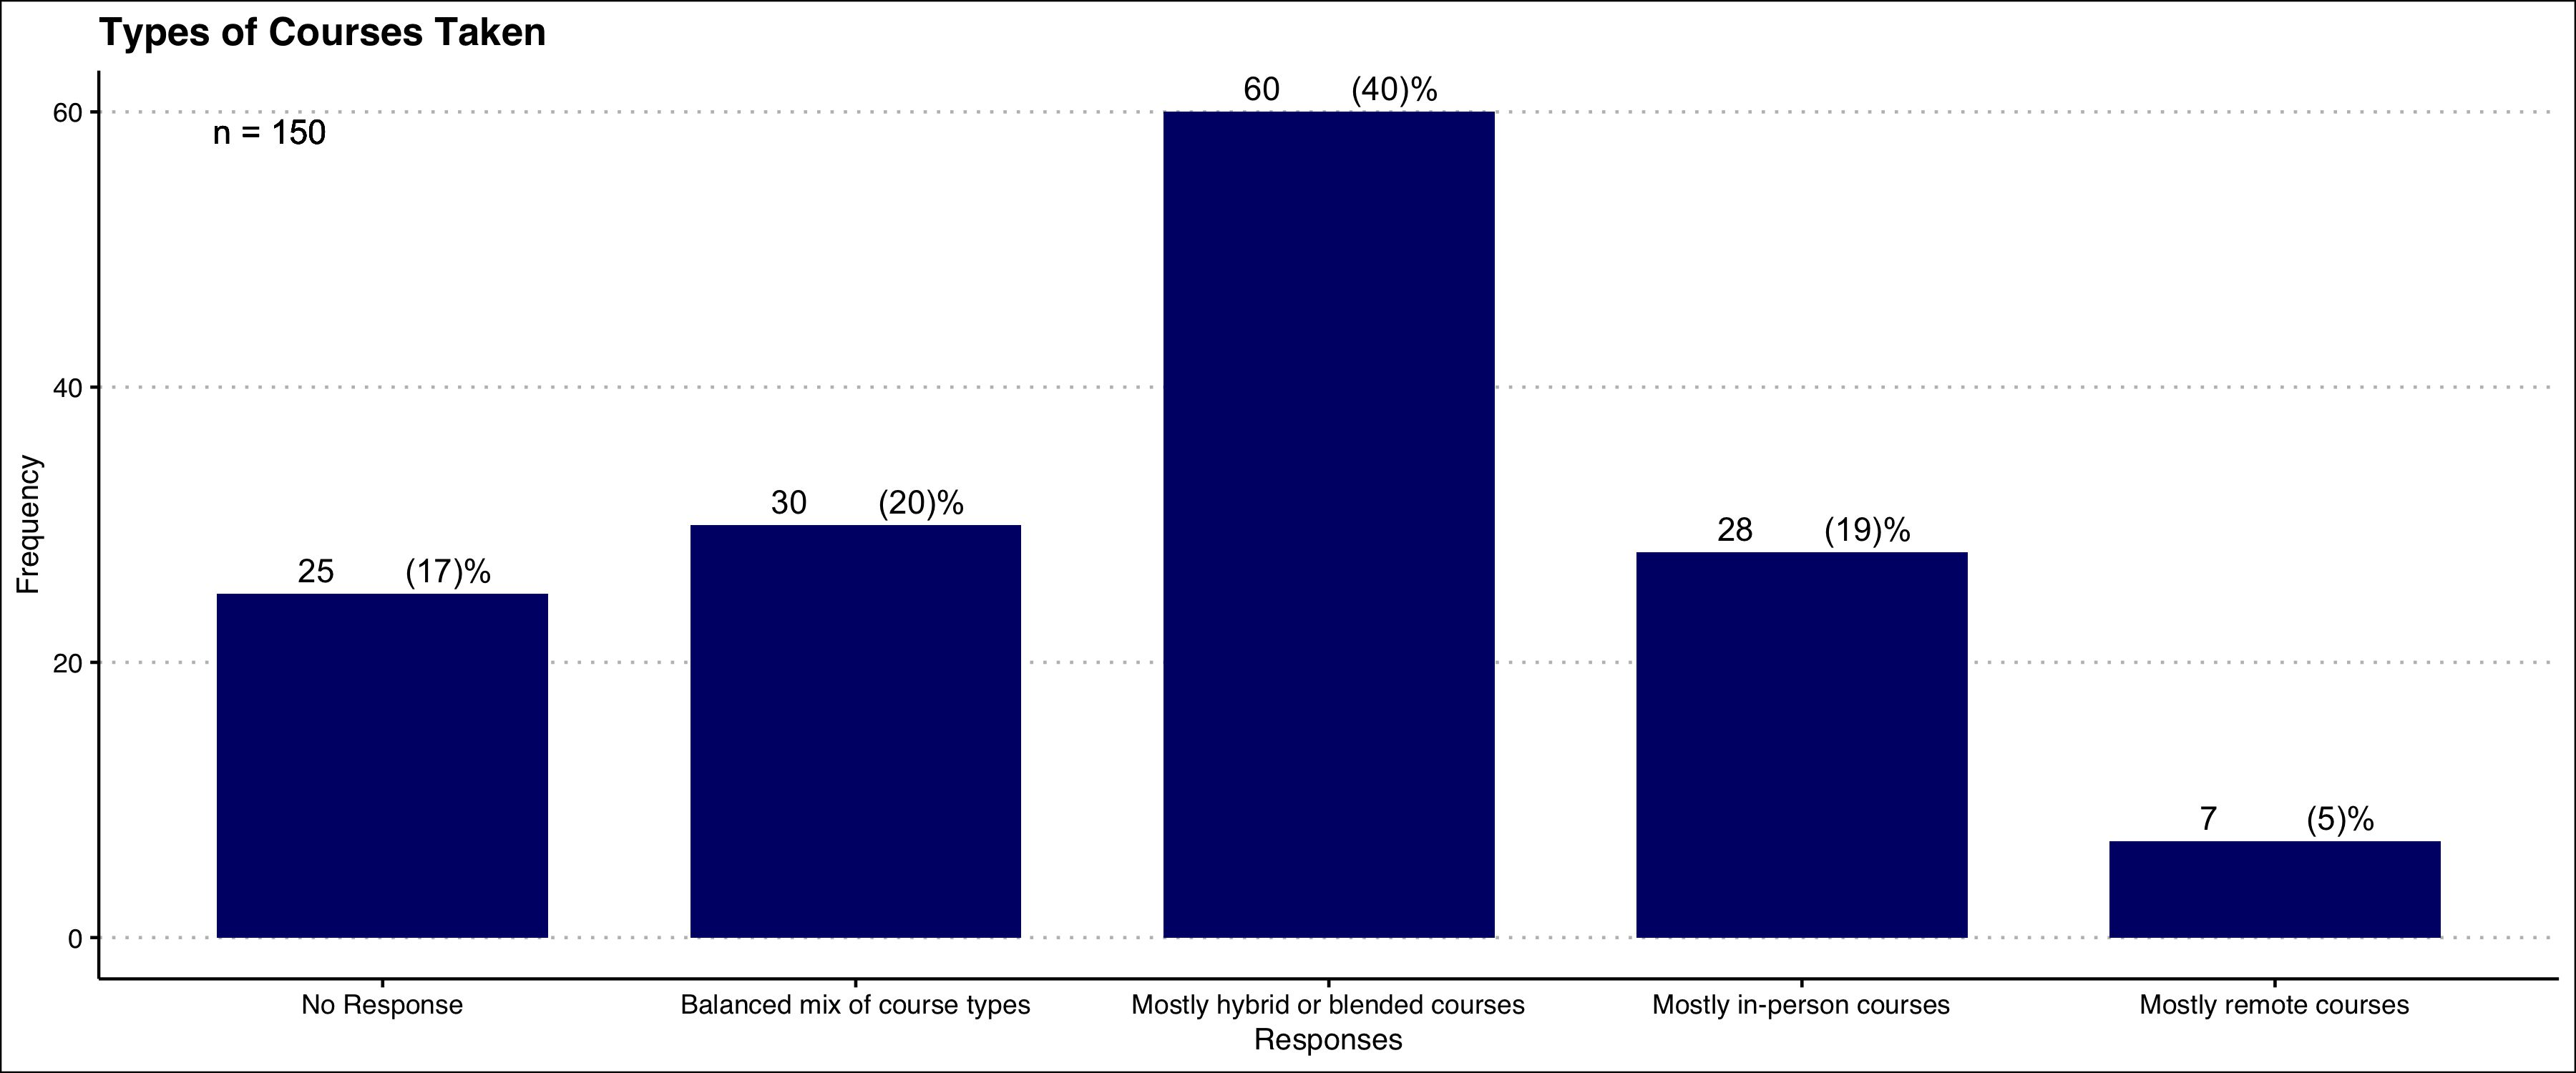
\includegraphics[width=\textwidth]{figures_4f06/types_of_courses_taken.jpg}
	\caption{Types of Courses Taken}
	\label{fig:2}
\end{figure}

Students were asked to reflect on their experiences as undergraduate students at McMaster University. Participants responded to two questions regarding how much coursework has emphasized certain aspects of their learning \figref{fig:3}, and how often they have applied their learning in different contexts \figref{fig:4}. 62

%%%%%During the current school year how much has your coursework emphasized the following
\begin{figure}[H]
	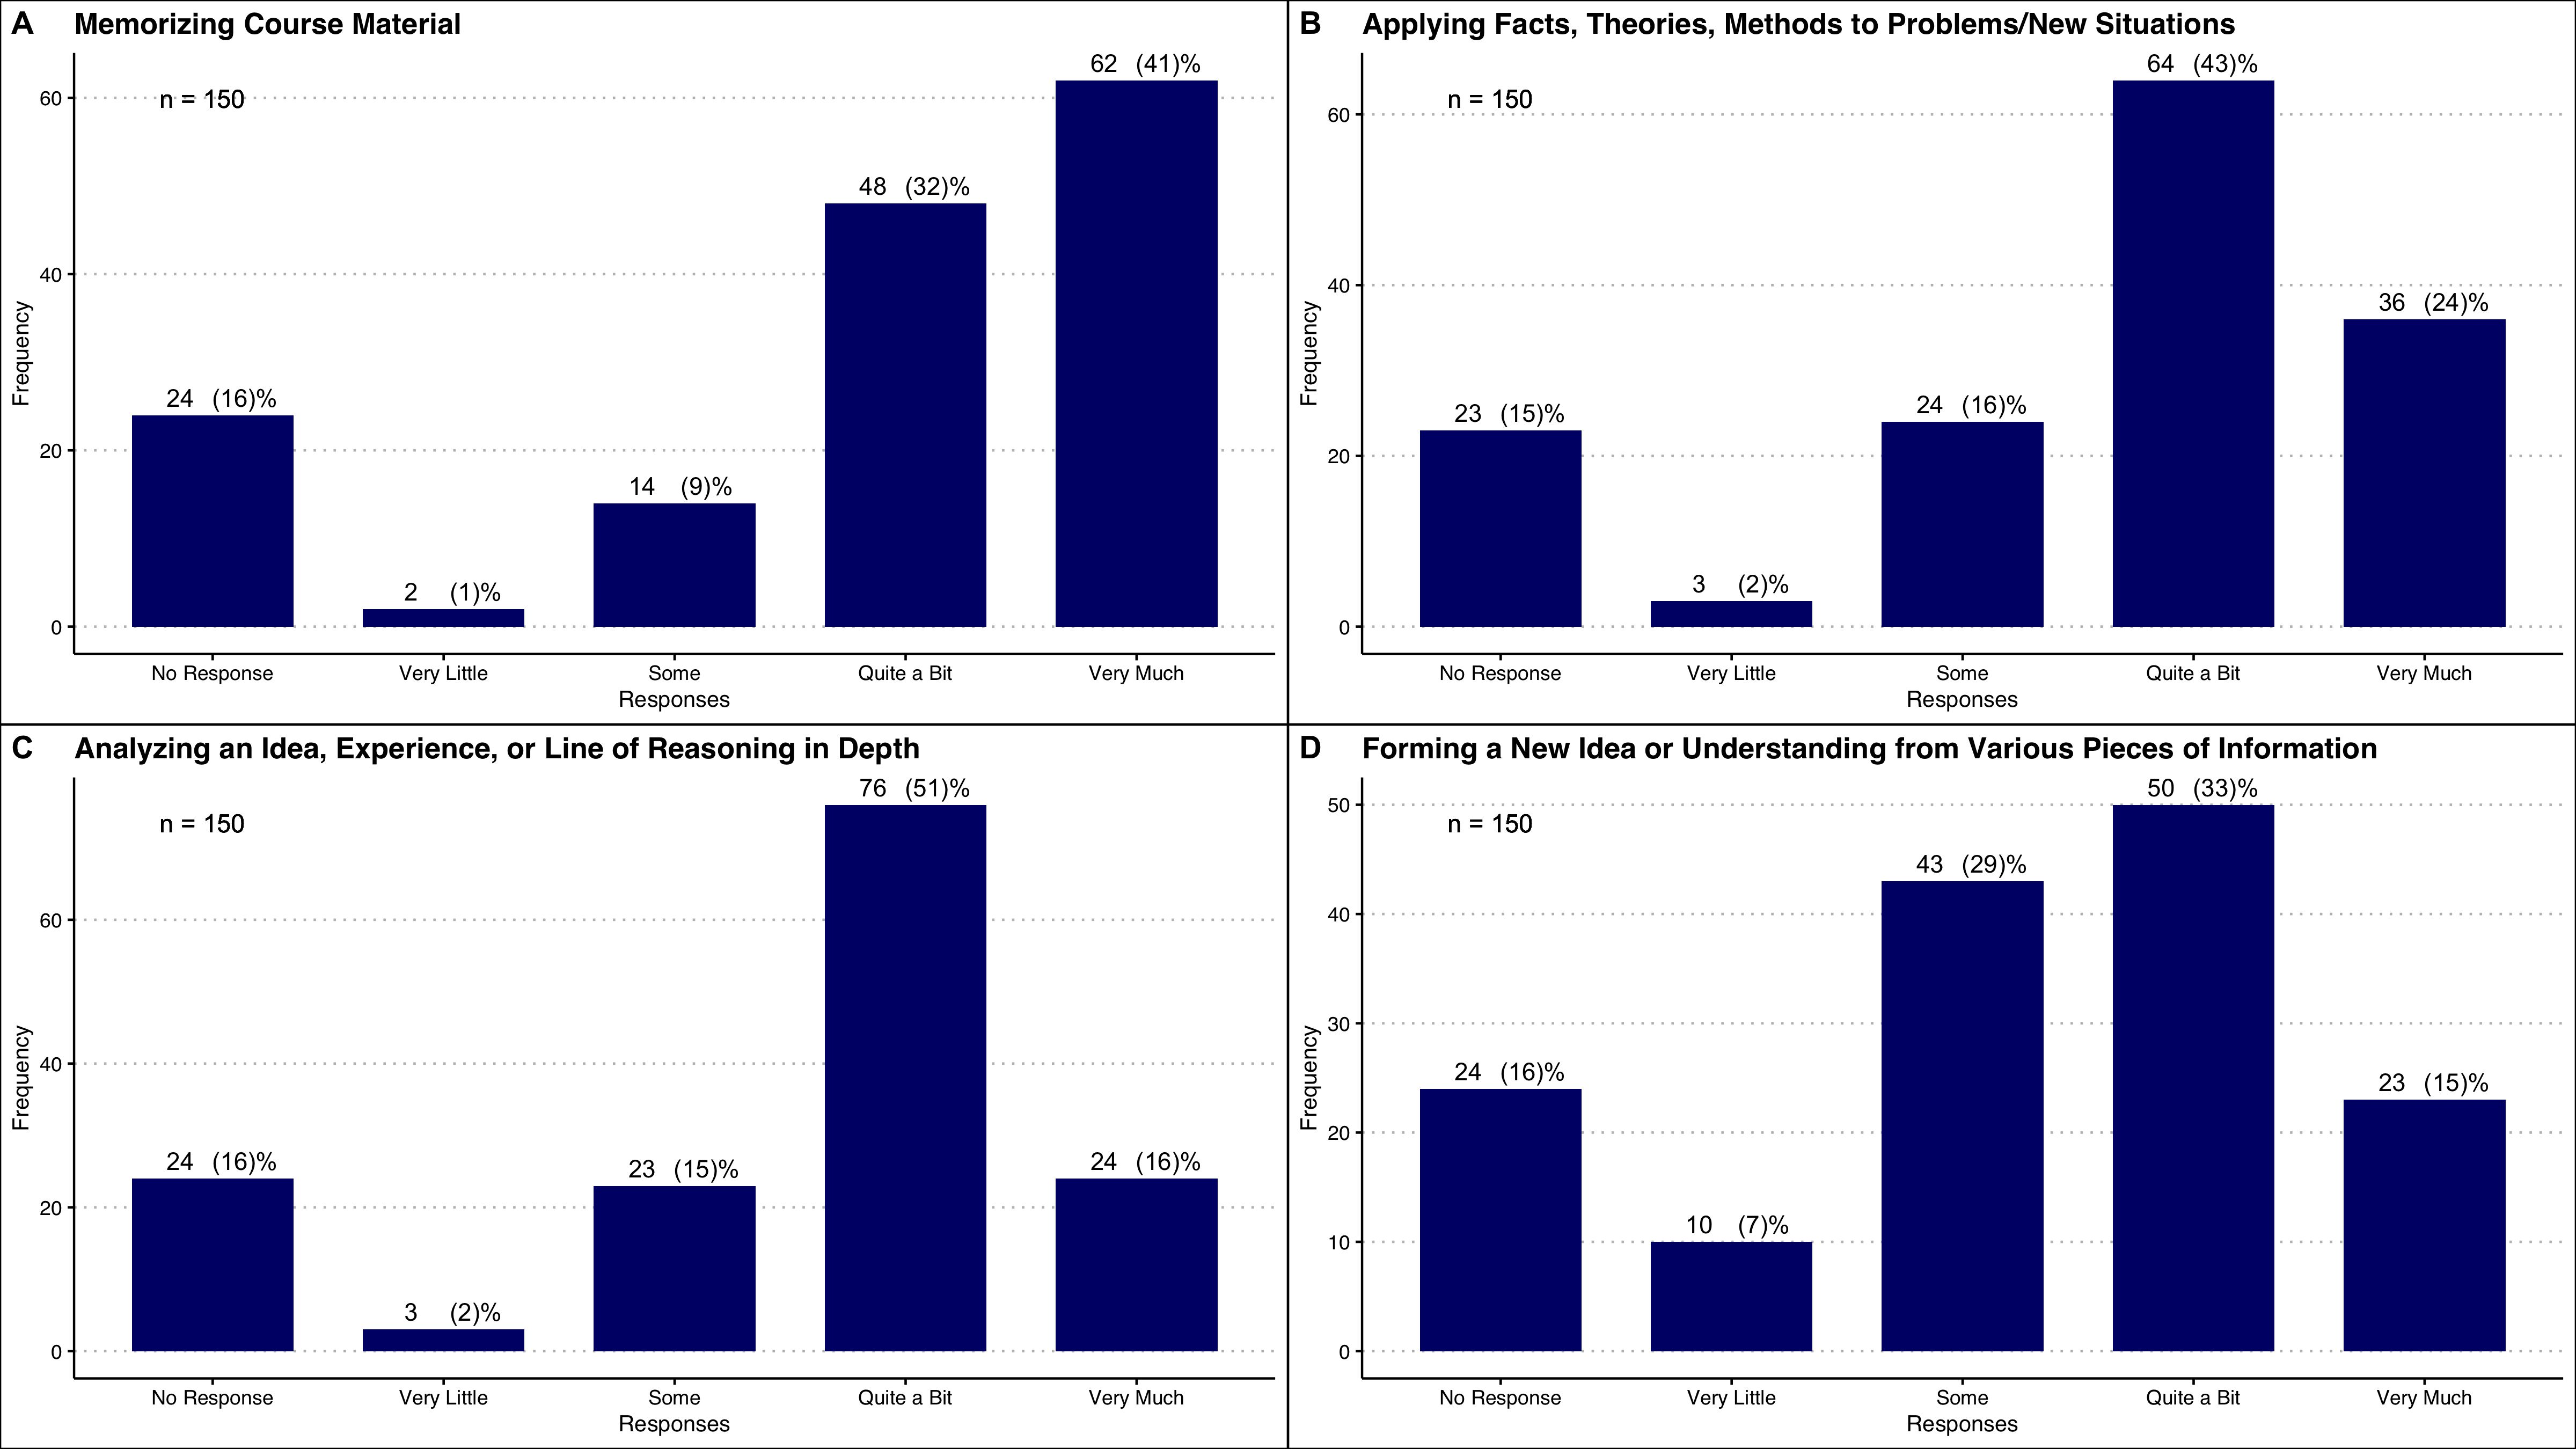
\includegraphics[width=\textwidth]{figures_4f06/howmuch_coursework_emphasized_thefollowing.jpg}
	\caption{How Much Has Coursework Emphasized the following}
	\label{fig:3}
\end{figure}

%%%%%During the current school year how often would you say you have done the following
\begin{figure}[H]
	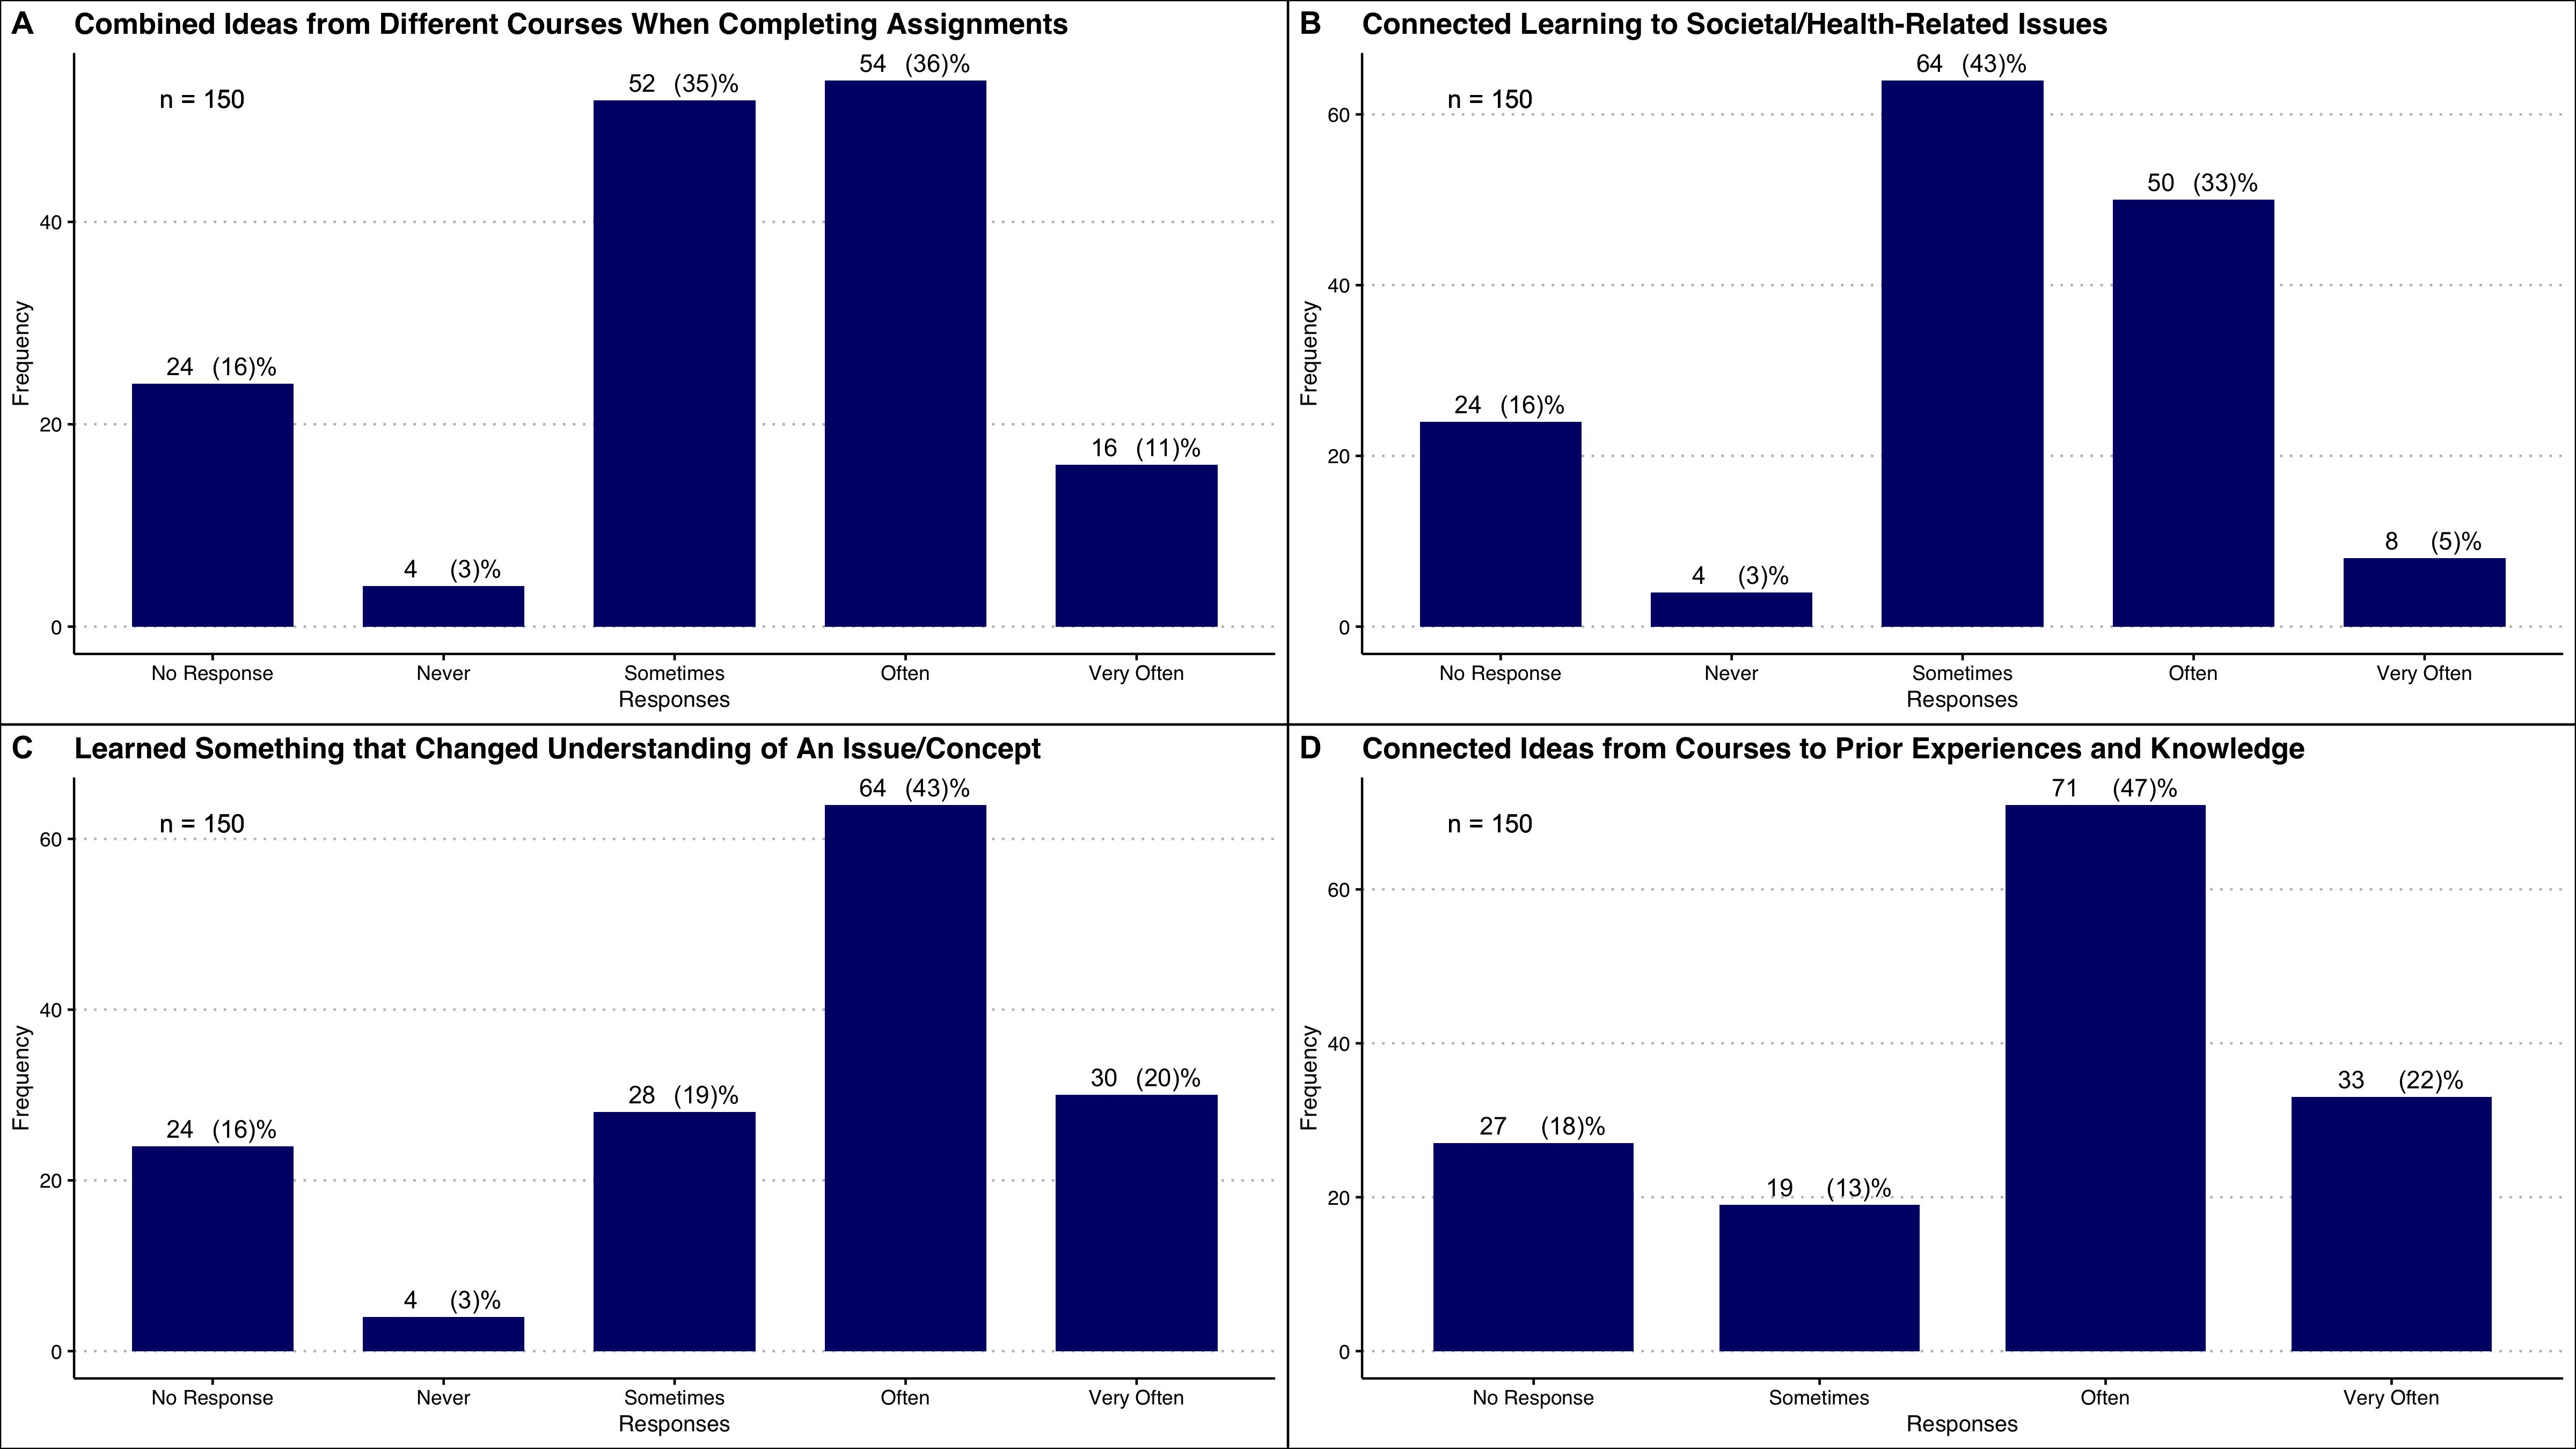
\includegraphics[width=\textwidth]{figures_4f06/how_often_haveyou_done_thefollowing.jpg}
	\caption{How often have you done the following}
	\label{fig:4}
\end{figure}

\subsection{Student perceptions on the use of game-based learning in biology}

%%%%%If game-based learning approaches were incorporated into one of your science courses, how do you think that this mode of learning can help with the following
\begin{figure}[H]
	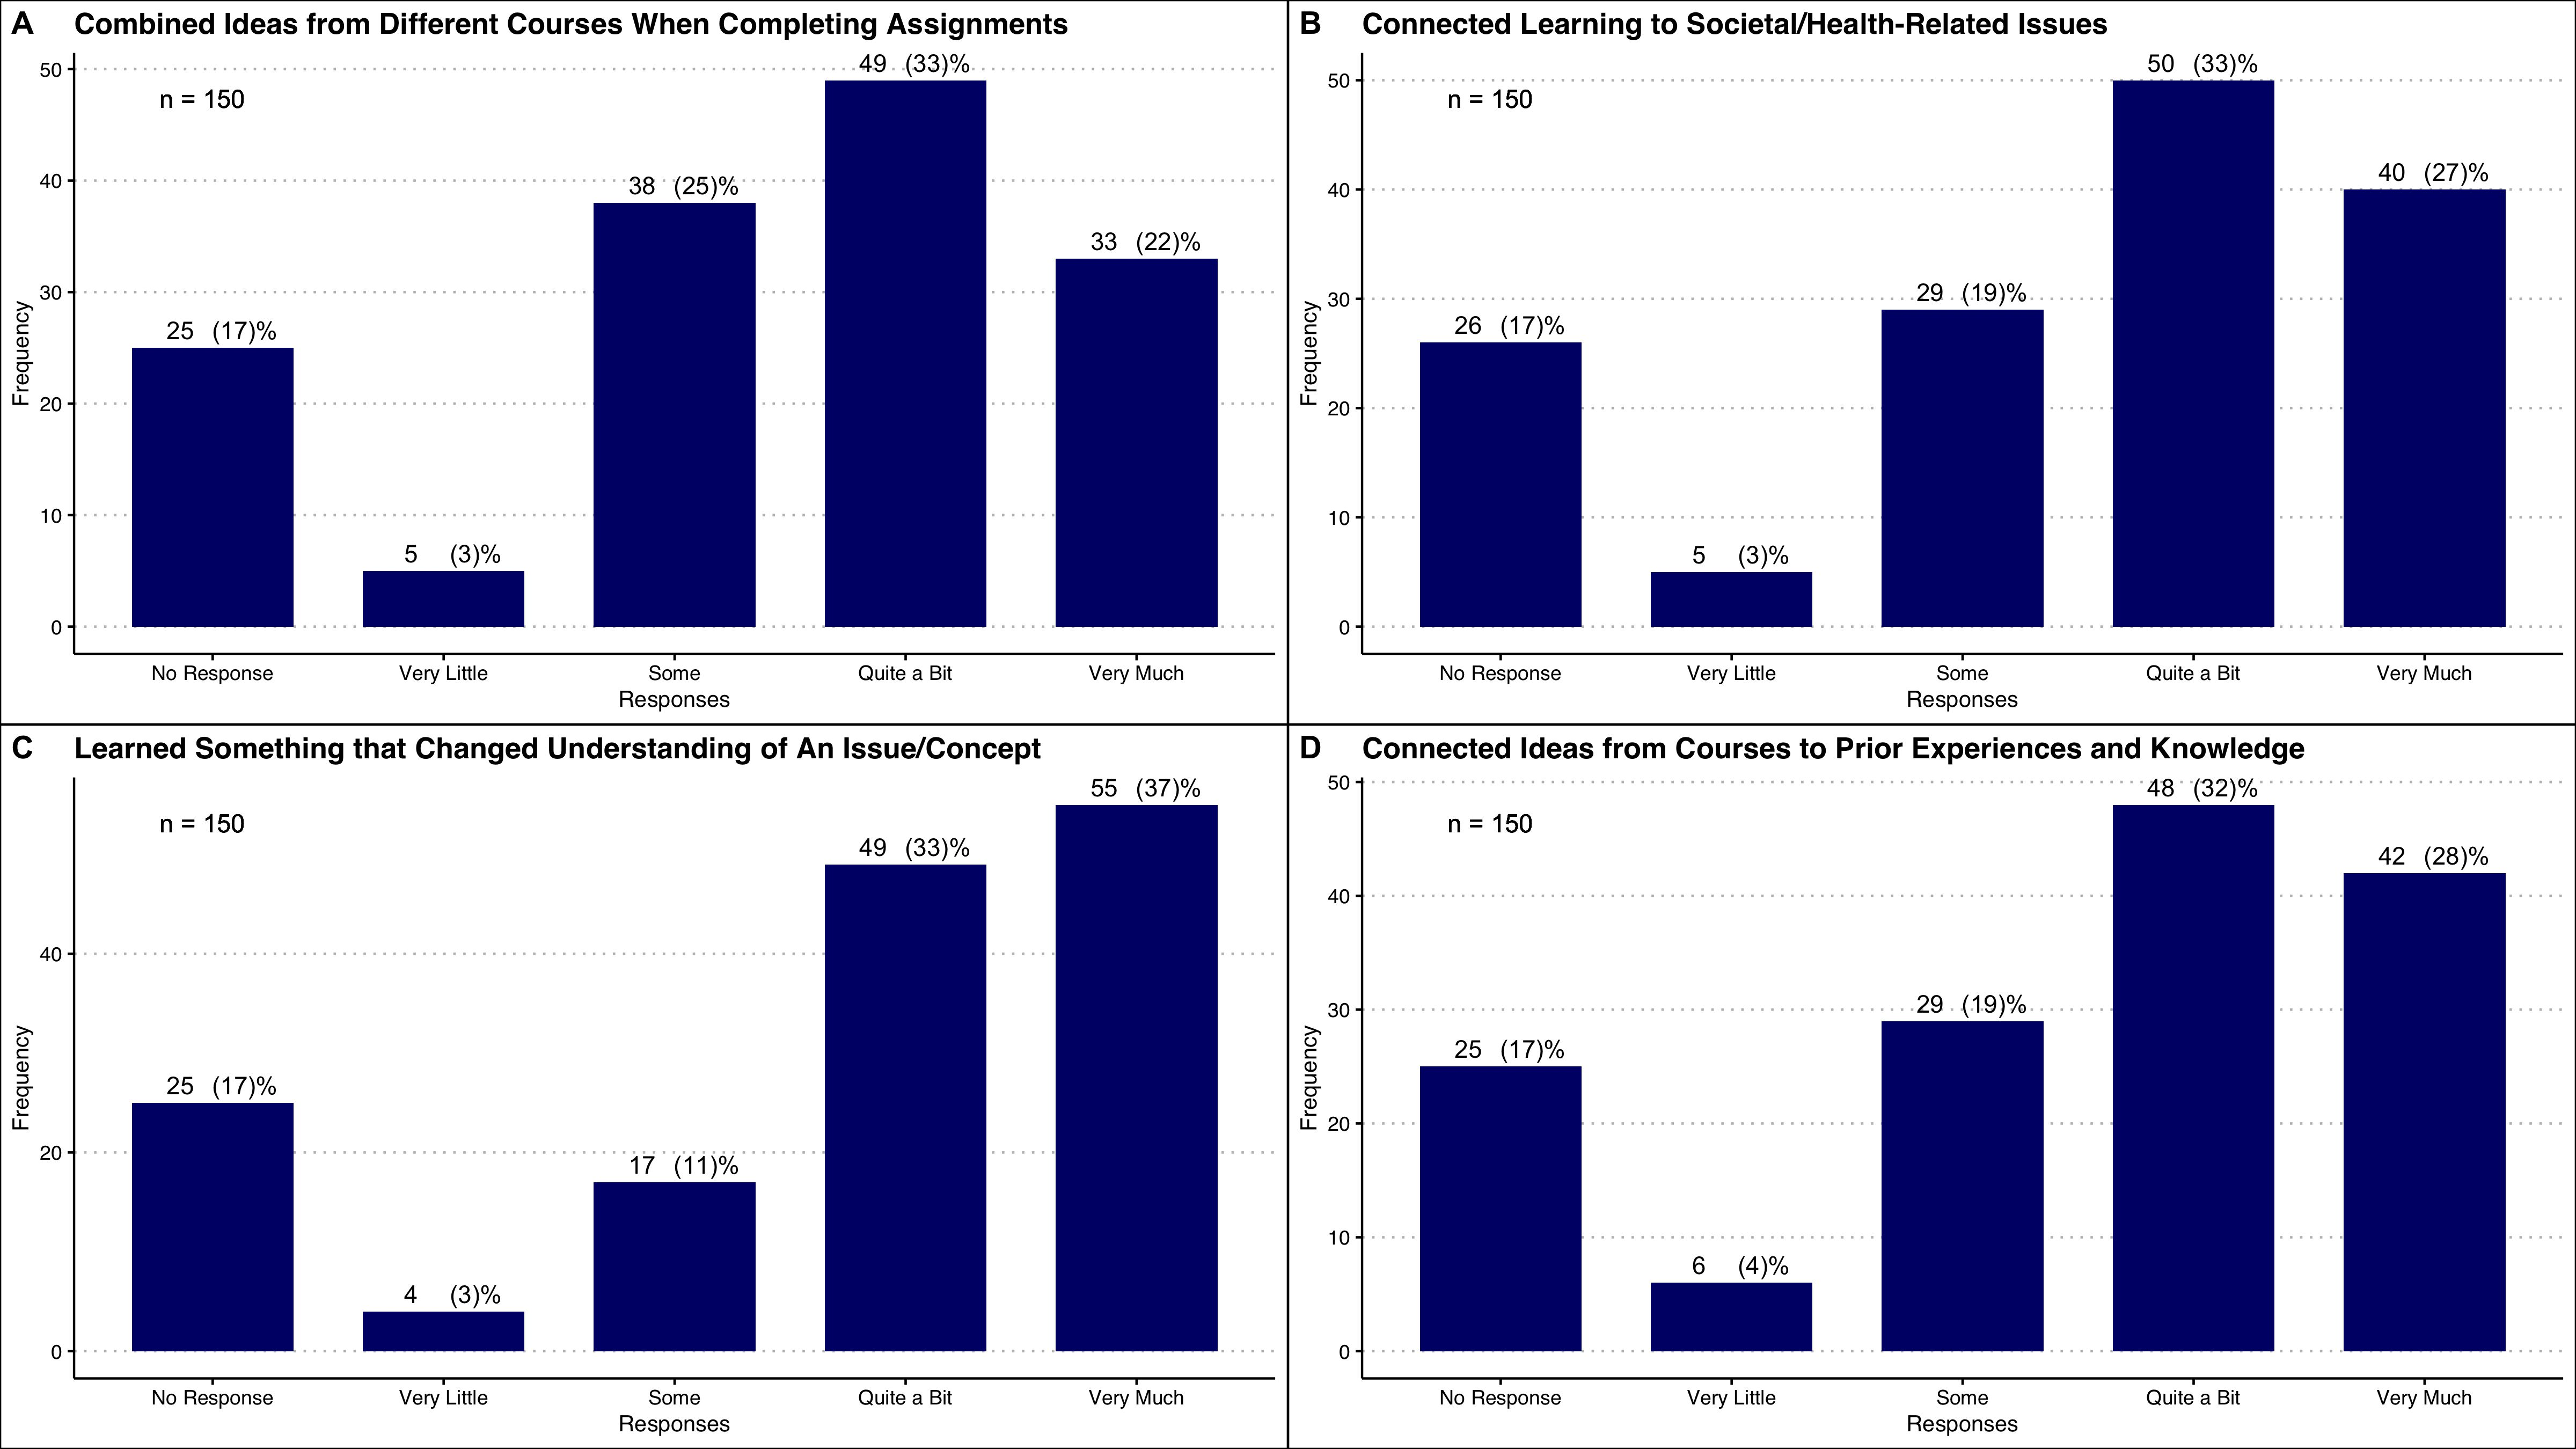
\includegraphics[width=\textwidth]{figures_4f06/how_does_gbl_help_in_science.jpg}
	\caption{If game-based learning approaches were incorporated in your science courses}
	\label{fig:5}
\end{figure}

%%%%% If BIO1A03 added a game-based learning component, how much would this improve your motivation to do the following?
\begin{figure}[H]
	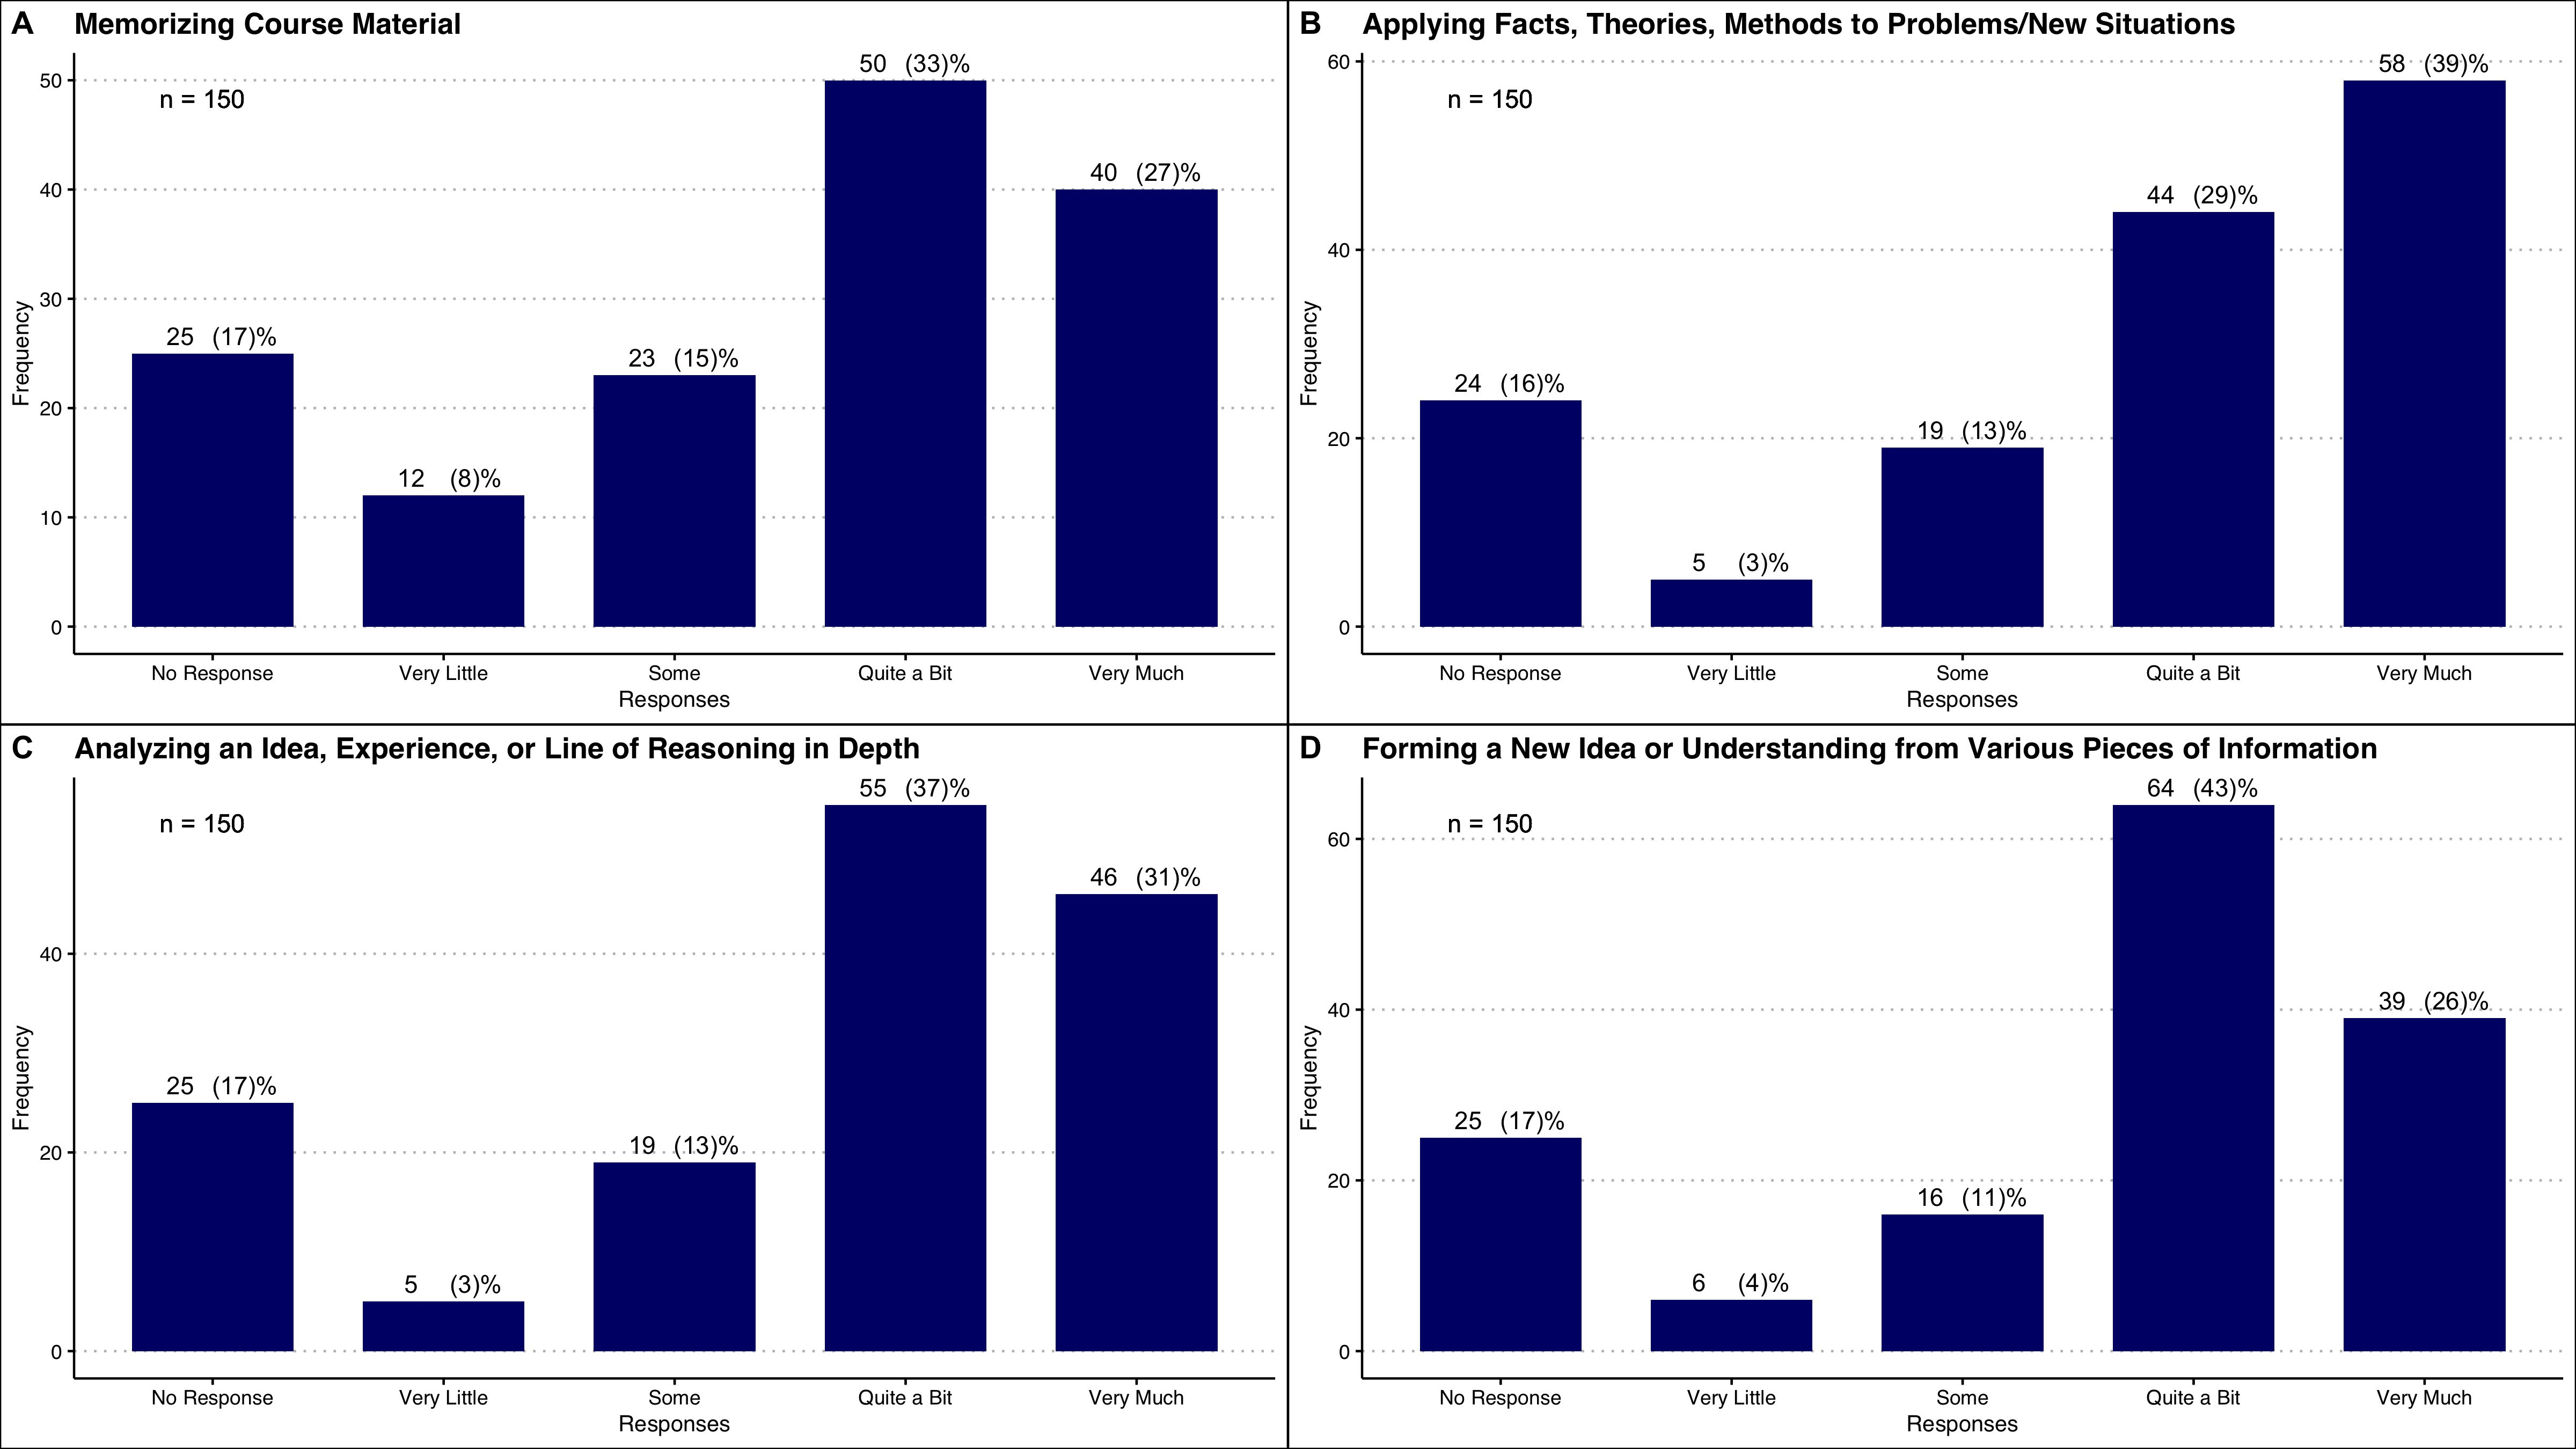
\includegraphics[width=\textwidth]{figures_4f06/ifbio1a03_added_gblcomponent.jpg}
	\caption{If BIO1A03 added a game-based component}
	\label{fig:6}
\end{figure}

%%%%% How likely is it that you would play the video game Cells at War on your own time, outside of class to further consolidate material taught during this class
\begin{figure}[H]
	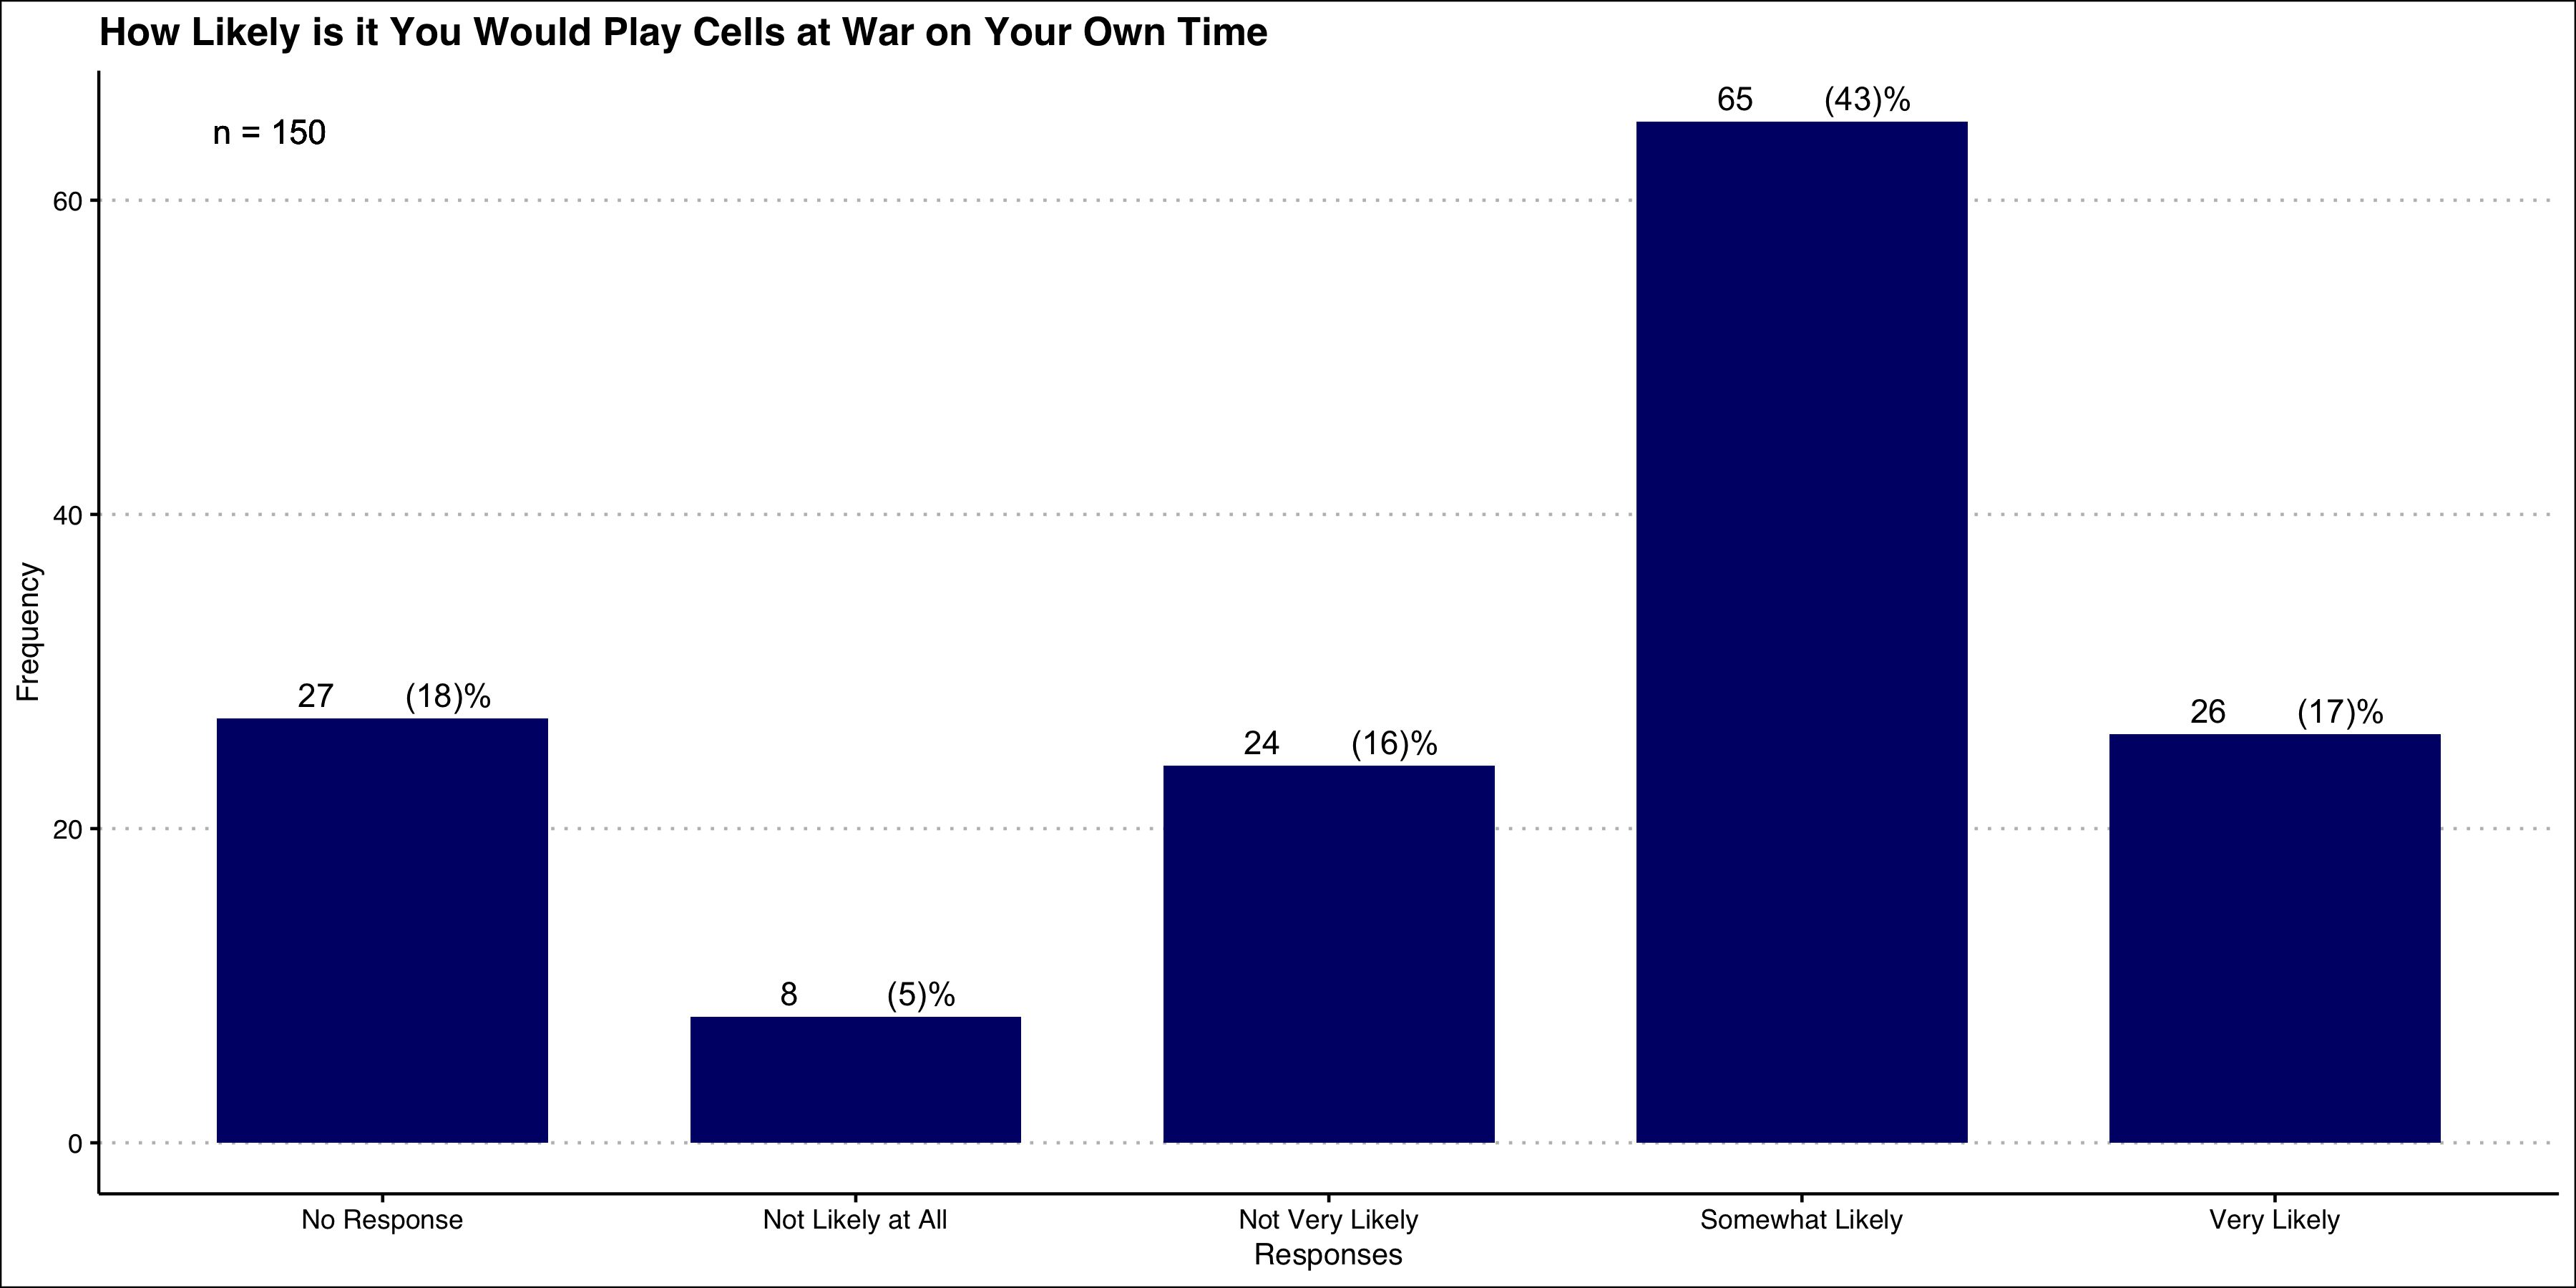
\includegraphics[width=\textwidth]{figures_4f06/how_likely_you_would_play_cellsatwar.jpg}
	\caption{How likely is it you would play Cells at War outside of class}
	\label{fig:7}
\end{figure}

%%%%%How prepared would you feel if you were given a quiz on Pompe Disease based on the Cells at War game, compared to studying off traditional lecture slides
\begin{figure}[H]
	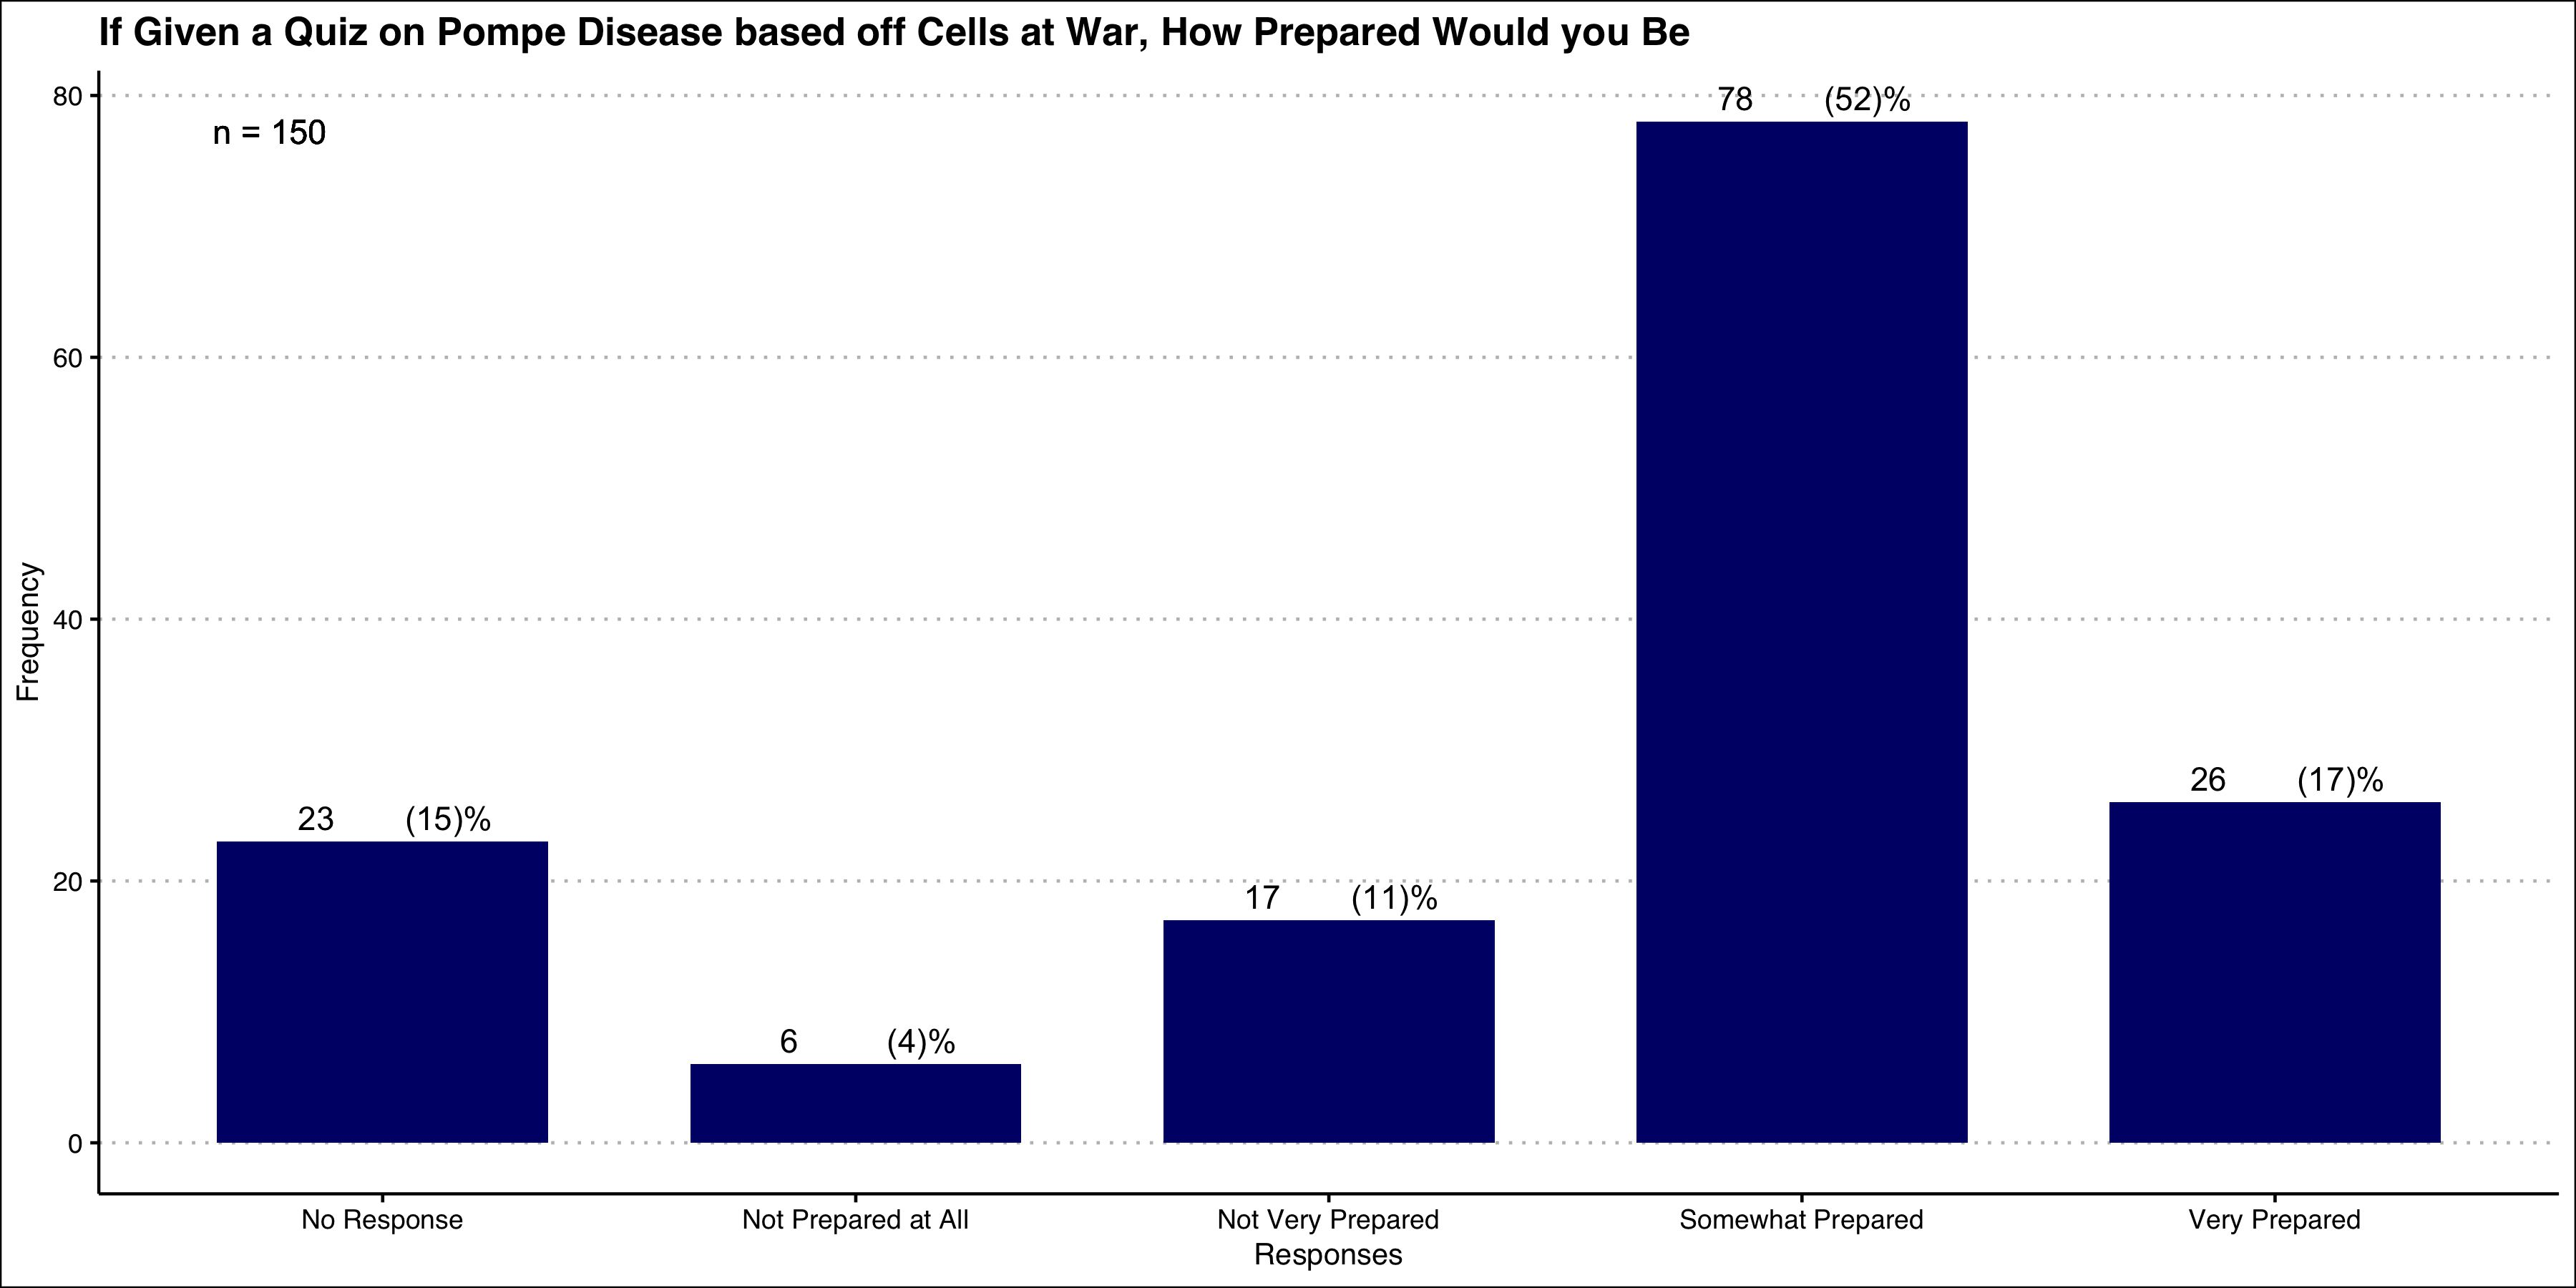
\includegraphics[width=\textwidth]{figures_4f06/how_prepared_if_tested_on_pompe_based_off_cellsatwar.jpg}
	\caption{How prepared would you feel if given a quiz on Pompe Disease}
	\label{fig:8}
\end{figure}

\section{Discussion}

We need to highlight in this section the use of Cells at War as an instructional tool as well as the benefits that students get out of this work integrated learning experience

\section{Future Directions}

\clearpage\newpage
\section{References}

%%%FIGURES%%%%%

%%%%PRINTING BIBLIOGRAPHY%%%%
\nocite{*}
\printbibliography[heading=none, sorting=nyt]
\newpage



\end{document}



